% Options for packages loaded elsewhere
\PassOptionsToPackage{unicode}{hyperref}
\PassOptionsToPackage{hyphens}{url}
%
\documentclass[
  english,
  man]{apa6}
\usepackage{lmodern}
\usepackage{amssymb,amsmath}
\usepackage{ifxetex,ifluatex}
\ifnum 0\ifxetex 1\fi\ifluatex 1\fi=0 % if pdftex
  \usepackage[T1]{fontenc}
  \usepackage[utf8]{inputenc}
  \usepackage{textcomp} % provide euro and other symbols
\else % if luatex or xetex
  \usepackage{unicode-math}
  \defaultfontfeatures{Scale=MatchLowercase}
  \defaultfontfeatures[\rmfamily]{Ligatures=TeX,Scale=1}
\fi
% Use upquote if available, for straight quotes in verbatim environments
\IfFileExists{upquote.sty}{\usepackage{upquote}}{}
\IfFileExists{microtype.sty}{% use microtype if available
  \usepackage[]{microtype}
  \UseMicrotypeSet[protrusion]{basicmath} % disable protrusion for tt fonts
}{}
\makeatletter
\@ifundefined{KOMAClassName}{% if non-KOMA class
  \IfFileExists{parskip.sty}{%
    \usepackage{parskip}
  }{% else
    \setlength{\parindent}{0pt}
    \setlength{\parskip}{6pt plus 2pt minus 1pt}}
}{% if KOMA class
  \KOMAoptions{parskip=half}}
\makeatother
\usepackage{xcolor}
\IfFileExists{xurl.sty}{\usepackage{xurl}}{} % add URL line breaks if available
\IfFileExists{bookmark.sty}{\usepackage{bookmark}}{\usepackage{hyperref}}
\hypersetup{
  pdftitle={Factor Loading Recovery for Smoothed Non-positive Definite Correlation Matrices},
  pdfauthor={Justin D. Kracht1},
  pdflang={en-EN},
  pdfkeywords={matrix smoothing, item factor analysis, factor loading recovery, indefinite},
  hidelinks,
  pdfcreator={LaTeX via pandoc}}
\urlstyle{same} % disable monospaced font for URLs
\usepackage{graphicx,grffile}
\makeatletter
\def\maxwidth{\ifdim\Gin@nat@width>\linewidth\linewidth\else\Gin@nat@width\fi}
\def\maxheight{\ifdim\Gin@nat@height>\textheight\textheight\else\Gin@nat@height\fi}
\makeatother
% Scale images if necessary, so that they will not overflow the page
% margins by default, and it is still possible to overwrite the defaults
% using explicit options in \includegraphics[width, height, ...]{}
\setkeys{Gin}{width=\maxwidth,height=\maxheight,keepaspectratio}
% Set default figure placement to htbp
\makeatletter
\def\fps@figure{htbp}
\makeatother
\setlength{\emergencystretch}{3em} % prevent overfull lines
\providecommand{\tightlist}{%
  \setlength{\itemsep}{0pt}\setlength{\parskip}{0pt}}
\setcounter{secnumdepth}{-\maxdimen} % remove section numbering
% Make \paragraph and \subparagraph free-standing
\ifx\paragraph\undefined\else
  \let\oldparagraph\paragraph
  \renewcommand{\paragraph}[1]{\oldparagraph{#1}\mbox{}}
\fi
\ifx\subparagraph\undefined\else
  \let\oldsubparagraph\subparagraph
  \renewcommand{\subparagraph}[1]{\oldsubparagraph{#1}\mbox{}}
\fi
% Manuscript styling
\usepackage{upgreek}
\captionsetup{font=singlespacing,justification=justified}

% Table formatting
\usepackage{longtable}
\usepackage{lscape}
% \usepackage[counterclockwise]{rotating}   % Landscape page setup for large tables
\usepackage{multirow}		% Table styling
\usepackage{tabularx}		% Control Column width
\usepackage[flushleft]{threeparttable}	% Allows for three part tables with a specified notes section
\usepackage{threeparttablex}            % Lets threeparttable work with longtable

% Create new environments so endfloat can handle them
% \newenvironment{ltable}
%   {\begin{landscape}\begin{center}\begin{threeparttable}}
%   {\end{threeparttable}\end{center}\end{landscape}}
\newenvironment{lltable}{\begin{landscape}\begin{center}\begin{ThreePartTable}}{\end{ThreePartTable}\end{center}\end{landscape}}

% Enables adjusting longtable caption width to table width
% Solution found at http://golatex.de/longtable-mit-caption-so-breit-wie-die-tabelle-t15767.html
\makeatletter
\newcommand\LastLTentrywidth{1em}
\newlength\longtablewidth
\setlength{\longtablewidth}{1in}
\newcommand{\getlongtablewidth}{\begingroup \ifcsname LT@\roman{LT@tables}\endcsname \global\longtablewidth=0pt \renewcommand{\LT@entry}[2]{\global\advance\longtablewidth by ##2\relax\gdef\LastLTentrywidth{##2}}\@nameuse{LT@\roman{LT@tables}} \fi \endgroup}

% \setlength{\parindent}{0.5in}
% \setlength{\parskip}{0pt plus 0pt minus 0pt}

% \usepackage{etoolbox}
\makeatletter
\patchcmd{\HyOrg@maketitle}
  {\section{\normalfont\normalsize\abstractname}}
  {\section*{\normalfont\normalsize\abstractname}}
  {}{\typeout{Failed to patch abstract.}}
\patchcmd{\HyOrg@maketitle}
  {\section{\protect\normalfont{\@title}}}
  {\section*{\protect\normalfont{\@title}}}
  {}{\typeout{Failed to patch title.}}
\makeatother
\shorttitle{Factor Loading Recovery for Smoothed Matrices}
\keywords{matrix smoothing, item factor analysis, factor loading recovery, indefinite\newline\indent Word count: X}
\DeclareDelayedFloatFlavor{ThreePartTable}{table}
\DeclareDelayedFloatFlavor{lltable}{table}
\DeclareDelayedFloatFlavor*{longtable}{table}
\makeatletter
\renewcommand{\efloat@iwrite}[1]{\immediate\expandafter\protected@write\csname efloat@post#1\endcsname{}}
\makeatother
\usepackage{lineno}

\linenumbers
\usepackage{csquotes}
\usepackage[titles]{tocloft}
\cftpagenumbersoff{figure}
\renewcommand{\cftfigpresnum}{\itshape\figurename\enspace}
\renewcommand{\cftfigaftersnum}{.\space}
\setlength{\cftfigindent}{0pt}
\setlength{\cftafterloftitleskip}{0pt}
\settowidth{\cftfignumwidth}{Figure 10.\qquad}
\cftpagenumbersoff{table}
\renewcommand{\cfttabpresnum}{\itshape\tablename\enspace}
\renewcommand{\cfttabaftersnum}{.\space}
\setlength{\cfttabindent}{0pt}
\setlength{\cftafterloftitleskip}{0pt}
\settowidth{\cfttabnumwidth}{Table 10.\qquad}
\usepackage{longtable, rotating}
\DeclareMathOperator{\tr}{tr}
\ifxetex
  % Load polyglossia as late as possible: uses bidi with RTL langages (e.g. Hebrew, Arabic)
  \usepackage{polyglossia}
  \setmainlanguage[]{english}
\else
  \usepackage[shorthands=off,main=english]{babel}
\fi

\title{Factor Loading Recovery for Smoothed Non-positive Definite Correlation Matrices}
\author{Justin D. Kracht\textsuperscript{1}}
\date{}


\affiliation{\vspace{0.5cm}\textsuperscript{1} University of Minnesota}

\abstract{
Researchers commonly use tetrachoric correlation matrices in item factor analysis. Unfortunately, tetrachoric correlation matrices are often non-positive definite (i.e., having one or more negative eigenvalues). These indefinite correlation matrices are problematic because the corresponding population correlation matrices they estimate are definitionally positive semidefinite (PSD; i.e., having strictly non-negative eigenvalues). Therefore, when used in procedures such as factor analysis, indefinite tetrachoric correlation matrices may result in poor estimates of factor loadings. Matrix smoothing algorithms attempt to remedy this problem by finding a PSD correlation matrix that is close, in some sense, to a given indefinite correlation matrix. However, little research has been done on the effectiveness of matrix smoothing. In the present simulation study, indefinite tetrachoric correlation matrices were calculated from simulated binary data sets. Three matrix smoothing algorithms---the Higham (2002), Bentler-Yuan (2011), and Knol-Berger algorithms (1991)---were applied to the indefinite tetrachoric correlation matrices. Factor analysis was then conducted on the smoothed and unsmoothed correlation matrices. The results show that smoothed matrices were slightly better estimates of their population counterparts compared to unsmoothed indefinite correlation matrices. However, using smoothed compared to unsmoothed indefinite correlation matrices for item factor analysis did not meaningfully improve factor loading recovery. Matrix smoothing should therefore be considered only as a tool to facilitate factor analysis of indefinite correlation matrices and not as a statistical remedy for the root causes of matrix indefiniteness.
}



\begin{document}
\maketitle

\newcommand{\Rsm}{\mathbf{R}_{\textrm{Sm}}}
\newcommand{\Rpop}{\mathbf{R}_{\textrm{Pop}}}
\newcommand{\Rnpd}{\mathbf{R}_{-}}
\newcommand{\Rapa}{\mathbf{R}_{\textrm{APA}}}
\newcommand{\Rby}{\mathbf{R}_{\textrm{BY}}}
\newcommand{\Rkb}{\mathbf{R}_{\textrm{KB}}}
\newcommand{\dg}{\textrm{dg}}
\newcommand{\RMSE}{\textrm{RMSE}(\mathbf{\Lambda}, \hat{\mathbf{\Lambda}})}

Tetrachoric correlation matrices (Olsson, 1979) are used to estimate the correlations between the normally-distributed, continuous latent variables assumed to underlie observed binary data. Therefore, tetrachoric correlation matrices are often recommended for use in item factor analysis because the common linear factor model requires the assumption that outcomes are continuous (Wirth \& Edwards, 2007). Unfortunately, tetrachoric correlation matrices are frequently \emph{indefinite}, having one or more negative eigenvalues (Bock, Gibbons, \& Muraki, 1988; Wothke, 1993). Indefinite correlation matrices are problematic because proper correlation matrices are, by definition, positive semi-definite (PSD; i.e., having all eigenvalues greater than or equal to 0; Wothke, 1993). Although indefinite correlation matrices resemble proper correlation matrices in many ways---they are symmetric, have unit diagonals, and all off-diagonal elements \(|r_{ij}| \leq 1\)---it is impossible to obtain an indefinite matrix of Pearson correlations from complete data. Thus, indefinite correlation matrices are improper estimates of their corresponding population correlation matrices in the sense that they are not included in the set of possible population correlation matrices.

Some researchers have suggested that one approach to resolving the problem of indefinite tetrachoric correlation matrices is to obtain a PSD correlation matrix that can be reasonably substituted for an indefinite tetrachoric correlation matrix (e.g., Devlin, Gnanadesikan, \& Kettenring, 1975; Dong, 1985). This approach is often referred to as \emph{matrix smoothing} and many algorithms developed for this purpose, referred to as \emph{matrix smoothing algorithms} (or simply, \emph{smoothing algorithms}), have been proposed in the psychometric literature and elsewhere (Bentler \& Yuan, 2011; Devlin et al., 1975; Dong, 1985; Fushiki, 2009; Higham, 2002; Knol \& Berger, 1991; Li, Li, \& Qi, 2010; Lurie \& Goldberg, 1998; Qi \& Sun, 2006). However, despite the the frequent occurrence of indefinite tetrachoric correlation matrices in psychometric research (Bock et al., 1988, p. 261), the variety of smoothing algorithms available, and suggestions to use matrix smoothing algorithms as a remedy to indefinite tetrachoric correlation matrices (Bentler \& Yuan, 2011; Knol \& Berger, 1991; Wothke, 1993), scant research has been done on the effectiveness of matrix smoothing algorithms in the context of item factor analysis of indefinite tetrachoric correlation matrices. In one of the only published comparisons of this kind, Knol and Berger (1991) investigated the effects of using smoothed compared to unsmoothed correlation matrices in factor analysis and found no large differences. However, this comparison was not a main focus of their study and only compared a small number of indefinite matrices (10 indefinite correlation matrices with 250 subjects and 15 items).

Moreover, few studies have compared the relative performance of matrix smoothing algorithms in the context of factor analysis (Debelak \& Tran, 2013, 2016). Debelak and Tran (2013) conducted a simulation study to determine which of three matrix smoothing algorithms --- the Higham Alternating Projections algorithm (APA; 2002), Bentler-Yuan algorithm (BY; 2011), and the Knol-Berger (KB; 1991) algorithm --- most often recovered the underlying dimensionality when applied to indefinite tetrachoric correlation matrices prior to parallel analysis (Horn, 1965). Debelak and Tran simulated binary data using a two-parameter logistic (2PL) item response theory (IRT; Birnbaum, 1968; de Ayala, 2013) model for one- and two-factor models with varying factor correlations, item difficulties, item discriminations, numbers of items, and numbers of subjects. Debelak and Tran then computed tetrachoric correlation matrices for each simulated binary data set. If a tetrachoric correlation matrix was indefinite, the three aforementioned smoothing algorithms were applied (resulting in three smoothed correlation matrices in addition to the indefinite tetrachoric matrix). Finally, Debelak and Tran conducted parallel analysis using each of these four correlation matrices to obtain estimates of dimensionality. Debelak and Tran concluded that \enquote{{[}the{]} application of smoothing algorithms generally improved correct identification of dimensionality when the correlation between the latent dimensions was 0.0 or 0.4 in our simulations} (Debelak \& Tran, 2013, p. 74). With respect to the relative performance of the Higham, Bentler-Yuan, and Knol-Berger smoothing algorithms in this context, Debelak and Tran concluded that there were \enquote{minor differences in the performance of the three smoothing algorithms used in {[}the{]} study. In data sets with a clear dimensional structure\ldots the algorithm of Bentler and Yuan (2011) performed best} (Debelak \& Tran, 2013, p. 74).

Following on these results, Debelak and Tran (2016) extended their simulation study design to evaluate the relative and absolute effectiveness of matrix smoothing algorithms when applied to indefinite polychoric correlation matrices of ordered, categorical (i.e., polytomous) data prior to conducting a parallel analysis. As in their previous study, Debelak and Tran used the accuracy of the parallel analysis dimensionality estimates (i.e., dimensionality recovery) as their evaluation criterion. In addition to extending their design to consider polytomous data, Debelak and Tran (2016) also considered factor models with either one or three major common factors and either zero or forty minor common factors. The minor common factors represented the effects of model approximation error; that is, the degree of model misfit inherent to mathematical models of natural phenomena in general, and psychological models in particular (MacCallum \& Tucker, 1991; MacCallum, Widaman, Preacher, \& Hong, 2001; Tucker, Koopman, \& Linn, 1969). Debelak and Tran concluded that the analysis of smoothed polychoric correlation matrices generally gave more accurate results than the analysis of indefinite polychoric correlation matrices. Moreover, they found that \enquote{methods based on the algorithms of Knol and Berger, Higham, and Bentler and Yuan showed a comparable performance with regard to the accuracy to detect the number of underlying major factors, with a slightly better performance of methods based on the Bentler and Yuan algorithm} (Debelak \& Tran, 2016, p. 15).

Both Debelak and Tran (2013) and Debelak and Tran (2016) concluded that the Bentler-Yuan (2011) smoothing algorithm led to the most accurate results (in terms of dimensionality recovery) when applied to indefinite tetrachoric or polychoric correlation matrices. However, neither study attempted to explain why the Bentler-Yuan algorithm led to better dimensionality recovery relative to the other smoothing methods they investigated. One intriguing possibility is that the smoothed correlation matrices produced by the Bentler-Yuan algorithm were better approximations of population correlation matrix than either the smoothed matrices produced by the Knol-Berger (1991) and Higham algorithms (2002), and also better approximations than the original indefinite tetrachoric or polychoric correlation matrices. If this is true, one might also expect that Bentler-Yuan smoothed tetrachoric correlation matrices will also lead to more accurate factor loading estimates compared to the alternatives.

The purpose of the present study was to address two questions related to these hypotheses. First, are smoothed indefinite tetrachoric correlation matrices better estimates of their corresponding population correlation matrices than the original indefinite tetrachoric correlation matrices and, if so, which smoothing method produces the best estimates? Second, do smoothed indefinite tetrachoric correlation matrices lead to better factor loading estimates compared to the unsmoothed tetrachoric matrices when used in exploratory factor analysis and, if so, which smoothing algorithm leads to the best factor loading estimates? To answer these questions, I conducted a simulation study in which I generated 124,346 indefinite tetrachoric correlation matrices from a variety of realistic data scenarios. Before describing the simulation design, I first introduce tetrachoric correlations, the three matrix smoothing algorithms under investigation, the common factor model, and the three factor analysis algorithms included in this study.

\hypertarget{tetrachoric-correlations}{%
\subsection{Tetrachoric Correlations}\label{tetrachoric-correlations}}

A tetrachoric correlation is an estimate of the linear association between two continuous, normally-distributed latent variables, \(y_1^*\) and \(y_2^*\) obtained using dichotomous, observed manifestations of those variables, \(y_1\) and \(y_2\). The variables \(y_1^*\) and \(y_2^*\) are assumed to follow a bivariate normal distribution,
\[
\left(\begin{array}{l}
y_{1}^* \\
y_{2}^*
\end{array}\right) \sim N\left[\left(\begin{array}{l}
0 \\
0
\end{array}\right),\left(\begin{array}{cc}
1 & r^* \\
r^* & 1
\end{array}\right)\right],
\]
where \(r^*\) is the true correlation between \(y_1^*\) and \(y_2^*\) that is estimated by the tetrachoric correlation, \(\hat{r}\). To compute the tetrachoric correlation, a \(2 \times 2\) contingency table is first created using \(y_1\) and \(y_2\) as described in Brown and Benedetti (1977). If any of the cell frequencies in the contingency table are zero, those elements are replaced with 0.5 and the other elements adjusted to leave the marginal sums unchanged (Brown \& Benedetti, 1977). The proportions of correct responses for \(y_1^*\) and \(y_2^*\) are represented by the marginals \(p_1\) and \(p_2\). The standard normal deviate thresholds \emph{h} and \emph{k} used to dichotomize \(y_1\) and \(y_2\) are then defined by \(F(h) = p_1\) and \(F(k) = p_2\) where \(F(z)\) is the area under the standard normal curve from 0 to \(\infty\) (Divgi, 1979). Given that \(y_1^*\) and \(y_2^*\) follow a bivariate normal distribution with correlation \(r\), \emph{h}, and \emph{k}, the likelihood function can be written as
\begin{equation}
L(h, k, r^{*})=\frac{1}{2 \pi \sqrt{1-r^{2}}} \int_{k}^{\infty} \int_{h}^{\infty} \exp \left(-\frac{y_1^{*2}+y_2^{*2}-2 r^* y_1^* y_2^*}{2\left(1-r^{*2}\right)}\right) d y_1^* d y_2^*.
\label{eq:likelihood-fn}
\end{equation}
The Newton-Raphson method can then be used to obtain successive approximations of \(r^*\) given an initial estimate, \(\hat{r}_0\):
\[
\hat{r}_{i + 1} = \hat{r}_i - \frac{L(h,k,\hat{r}_i) - p_{ii}}{L^\prime(h,k,\hat{r}_i)},
\]
where \(p_{11}\) is the proportion of correct responses on both \(y_1^*\) and \(y_2^*\) and \(L^\prime(h,k,\hat{r}_i)\) is the first derivative of \eqref{eq:likelihood-fn} (Divgi, 1979). Iteration continues until convergence is achieved (when \(\hat{r}_{i+1} - \hat{r}_i < \delta\) for some small value of delta) or until some maximum number of iterations occur. For \(p\) dichotomous variables, the \(p \times p\) symmetric matrix \(\mathbf{R}_{\textrm{Tet}}\) with a unit diagonal and off-diagonal elements consisting of pairwise tetrachoric correlation coefficients \(\hat{r}_{jk}, \: j,k \in \{1, \dots p \}\), is called the tetrachoric correlation matrix. Just as the tetrachoric correlation \(\hat{r}_{jk}\) estimates \(r^*_{jk}\), the tetrachoric correlation matrix \(\mathbf{R}_{\textrm{Tet}}\) estimates the \(p \times p\) population correlation matrix, \(\mathbf{R}_{\textrm{Pop}}\), which is symmetric with off-diagonal elements \(r^*_{jk}\), and a unit diagonal.

\hypertarget{matrix-smoothing-algorithms}{%
\subsection{Matrix Smoothing Algorithms}\label{matrix-smoothing-algorithms}}

\hypertarget{higham-alternating-projections-algorithm-apa-2002}{%
\subsubsection{Higham Alternating Projections Algorithm (APA; 2002)}\label{higham-alternating-projections-algorithm-apa-2002}}

The matrix smoothing algorithm proposed by Higham (2002) seeks to find the closest PSD correlation matrix to a given indefinite correlation matrix. In this context, closeness is defined as the generalized Euclidean distance (Banerjee \& Roy, 2014, p. 492). Higham's algorithm (2002) uses a series of alternating projections to locate the PSD correlation matrix (\(\mathbf{R}_{\textrm{APA}}\)) closest to a given indefinite correlation matrix (\(\mathbf{R}_{-}\)) of the same order. The algorithm works by first projecting \(\mathbf{R}_{-}\) onto the set of symmetric, PSD \(p \times p\) matrices, \(\mathcal{S}\). The resulting candidate matrix is then projected onto the set of symmetric \(p \times p\) matrices with unit diagonals, \(\mathcal{U}\). The series of projections repeats until the algorithm converges to a matrix, \(\mathbf{R}_{\textrm{APA}}\), that is PSD, symmetric, and has a unit diagonal, or until the maximum number of iterations is exceeded.

Specifically, Higham's algorithm (2002) consists of alternating projection functions, \(P_U\), the projection onto \(\mathcal{U}\), and \(P_S\), the projection onto \(\mathcal{S}\). For some symmetric \(\mathbf{A} \in \mathbb{R}^{p \times p}\) with elements \(a_{ij}\),
\begin{equation}
P_U(\mathbf{A}) = (p_{ij}), \: p_{ij} = 
\begin{cases}
\begin{aligned}
&a_{ij}, &i \neq j \\
&1, &i = j.
\end{aligned}
\end{cases}
\label{eq:proj-U}
\end{equation}
Stated simply, \(P_U(\mathbf{A})\) replaces all non-unit elements of the diagonal of \(\mathbf{A}\) with ones. The projection onto \(\mathcal{S}\) is less straightforward. Higham (2002) outlines the steps as follows. For some symmetric \(\mathbf{A} \in \mathbb{R}^{p \times p}\) let \(\mathbf{A} = \mathbf{V} \mathbf{\Lambda}_- \mathbf{V}^{\textrm{T}}\) be the eigendecomposition of \(\mathbf{A}\), where \(\mathbf{V}\) is the orthonormal matrix of eigenvectors and \(\mathbf{\Lambda_-} = \textrm{diag}(\lambda_i)\) is a diagonal matrix with the eigenvalues of \(\mathbf{A}\), \(\lambda_i, \: i \in \{1, \dots, p \}\), ordered from largest to smallest on the diagonal (\(\lambda_1 \geq \lambda_2 \geq \dots \geq \lambda_p\), \(\lambda_p < 0\)). Also let \(\mathbf{\Lambda}_+ = \textrm{diag}(\max(\lambda_i, 0))\). Then the projection of \(\mathbf{A}\) onto \(\mathcal{S}\) can be written as
\begin{equation}
P_S(\mathbf{A}) = \mathbf{V} \mathbf{\Lambda_+} \mathbf{V}^{\textrm{T}}.
\label{eq:proj-S}
\end{equation}
Starting with \(\mathbf{A} = \mathbf{R}_{-}\), \(\mathbf{R}_{\textrm{APA}}\) can be obtained by repeatedly applying the operation \(\mathbf{A} \leftarrow P_U(P_S(\mathbf{A}))\) until convergence occurs or until some maximum number of iterations is reached (Higham, 2002, p. 337).

\hypertarget{bentler-yuan-algorithm-by-2011}{%
\subsubsection{Bentler-Yuan Algorithm (BY; 2011)}\label{bentler-yuan-algorithm-by-2011}}

The Bentler-Yuan (2011) smoothing algorithm is based on minimum-trace factor analysis (MTFA; Bentler, 1972; Jamshidian \& Bentler, 1998). MTFA seeks to find optimal communality estimates such that unexplained common variance is minimized while constraining the diagonal matrix of unique variances and the observed covariance matrix with the estimated communalities as diagonal elements to be positive semidefinite (PSD). In contrast with the Higham algorithm (2002), the Bentler-Yuan algorithm does not seek to minimize some criterion. Instead, the algorithm uses MTFA to identify Heywood cases (i.e., communality estimates greater than or equal to one and, consequently, negative or zero uniqueness variance estimates; Dillon, Kumar, \& Mulani, 1987). The Bentler-Yuan algorithm then rescales the rows and columns of \(\mathbf{R}_{-}\) corresponding to these Heywood cases to produce a smoothed, PSD correlation matrix, \(\mathbf{R}_{\textrm{BY}}\). More specifically, the algorithm first conducts an MTFA using \(\mathbf{R}_{-}\). Using the results of the MTFA, a diagonal matrix, \(\mathbf{H}\) is constructed containing the estimated communalities as diagonal elements. Next, another diagonal matrix, \(\mathbf{\Delta}^2\), is constructed with elements \(\delta_i^2\) where \(\delta_i^2 = 1\) if \(h_i < 1\) and \(\delta_i^2 = k / h_i\) otherwise (where \(k < 1\) is some constant). Finally, the smoothed, PSD correlation matrix \(\mathbf{R}_{\textrm{BY}}= \mathbf{\Delta} \mathbf{R}_0 \mathbf{\Delta} + \mathbf{I}\) is obtained, where \(\mathbf{R}_0\) is \(\mathbf{R}_{-}\) with diagonal elements replaced by zeroes and \(\mathbf{I}\) is an identity matrix that ensures that \(\mathbf{R}_{\textrm{BY}}\) has a unit diagonal.

Similar to the Higham algorithm, the Bentler-Yuan algorithm sometimes fails to produce a PSD correlation matrix. This can happen either when (a) the MTFA algorithm fails to converge or (b) when \(k\) is too large and does not shrink the targeted elements of the indefinite correlation matrix enough for the matrix to become PSD. To help with this non-convergence, I used the modified Bentler-Yuan algorithm implementation provided by the \texttt{smoothBY()} function in the R \emph{fungible} package (Waller, 2019) to adaptively select an appropriate \(k\). The \(k\) parameter was initialized at \(k = 0.999\) and decreased by \(0.001\) until the algorithm produced a PSD correlation matrix or \(k = 0\).\footnote{Bentler and Yuan suggest using \(k = 0.96\) (Bentler \& Yuan, 2011, p. 120) but claim that the precise value of \(k\) does not matter a great deal as long as \(k\) is marginally less than one.}

\hypertarget{knol-berger-algorithm-kb-1991}{%
\subsubsection{Knol-Berger Algorithm (KB; 1991)}\label{knol-berger-algorithm-kb-1991}}

In contrast to the Higham (2002) and Bentler-Yuan (2011) smoothing algorithms, the Knol-Berger algorithm is a non-iterative procedure in which the negative eigenvalues of \(\mathbf{R}_{-}\) are replaced with some small positive value. The first step in the Knol-Berger algorithm is to compute the eigendecomposition of the \(p \times p\) indefinite correlation matrix, \(\mathbf{R}_{-}= \mathbf{V \Lambda V}^\prime\), where \(\mathbf{V}\) is an orthonormal matrix containing the eigenvectors of \(\mathbf{R}_{-}\) and \(\mathbf{\Lambda}\) is a diagonal matrix with the eigenvalues of \(\mathbf{R}_{-}\), \(\lambda_i, \: i \in \{1, \dots, p \}\), ordered from largest to smallest on the diagonal (\(\lambda_1 \leq \lambda_2 \leq \dots \leq \lambda_p\), \(\lambda_p < 0\)). Next, a matrix \(\mathbf{\Lambda_+}\) is created by setting all negative elements of \(\mathbf{\Lambda}\) equal to some user-specified small, positive constant. Finally, a smoothed, PSD correlation matrix, \(\mathbf{R}_{\textrm{KB}}\), is constructed by replacing \(\mathbf{\Lambda}\) with \(\mathbf{\Lambda_+}\) in the eigendecomposition of \(\mathbf{R}_{-}\) and then scaling to ensure a unit diagonal and all off-diagonal elements \(|r_{ij}| \leq 1\):

\begin{equation}
\mathbf{R}_{\textrm{KB}}= [\textrm{dg}(\mathbf{V \Lambda_+ V}^\prime)]^{-1/2} \mathbf{V \Lambda_+ V}^\prime \textrm{dg}(\mathbf{V \Lambda_+ V}^\prime)]^{-1/2},
\label{eq:Rkb}
\end{equation}

\hypertarget{the-common-factor-model}{%
\subsection{The Common Factor Model}\label{the-common-factor-model}}

The linear factor analysis model is used to describe the variance of each observed variable in terms of the contributions of a small number of latent common factors and a specific factor unique to that variable (Wirth \& Edwards, 2007). In the common factor model, the population correlation matrix, \(\mathbf{P}\), can be expressed as:

\begin{equation}
\mathbf{P} = \mathbf{F} \mathbf{\Phi} \mathbf{F}^{\prime} + \mathbf{\Theta}^2
\label{eq:cfa}
\end{equation}

where \(\mathbf{P}\) is a \(p \times p\) population correlation matrix for \(p\) observed variables, \(\mathbf{F}\) is a \(p \times m\) factor loading matrix for \(m\) common factors, \(\mathbf{\Phi}\) is an \(m \times m\) matrix of correlations between the \(m\) common factors, and \(\mathbf{\Theta}^2\) is a \(p \times p\) diagonal matrix containing the unique variances.

Although the common factor analysis model represented in \eqref{eq:cfa} is often useful, many authors have remarked that it constitutes an oversimplification of the complex processes that generate real, observed data (Cudeck \& Henly, 1991; MacCallum \& Tucker, 1991; MacCallum et al., 2001). Tucker, Koopman, and Linn (1969) suggested that the lack-of-fit between the common factor model and the complex processes underlying real data could be represented by modeling a large number of minor common factors of small effect. The model Tucker et al.~(1969) proposed can be written as:
\begin{equation}
\mathbf{P} = \mathbf{F} \mathbf{\Phi} \mathbf{F}^{\prime} + \mathbf{\Theta}^2 + \mathbf{WW}^{\prime}
\label{eq:cfa-error}
\end{equation}
where \(\mathbf{W}\) is a \(p \times q\) matrix containing factor loadings for the \(q \gg m\) minor factors (Briggs \& MacCallum, 2003, p. 32). Given our expectation that the common factor model is not a perfect representation of any real-world data-generating process we might wish to represent, \eqref{eq:cfa-error} should be preferred to \eqref{eq:cfa} for simulating realistic data (Briggs \& MacCallum, 2003; Hong, 1999).

\hypertarget{factor-analysis-algorithms}{%
\subsection{Factor Analysis Algorithms}\label{factor-analysis-algorithms}}

One purpose of this study was to determine whether the effects of matrix smoothing method on factor loading recovery differ depending on the factor analysis algorithm used. To that end, three factor analysis methods were used in the current simulation: principal axes (PA), ordinary least-squares (OLS), and maximum-likelihood (ML). These factor analysis methods were chosen because they are some of the most commonly used methods (Fabrigar, Wegener, MacCallum, \& Strahan, 1999) and because two of the methods (PA and OLS) work when an indefinite correlation matrix is given as input.

\hypertarget{principal-axes-factor-analysis}{%
\subsubsection{Principal Axes Factor Analysis}\label{principal-axes-factor-analysis}}

Principal axes (PA) factor analysis is conceptually similar to principal components analysis (PCA). Whereas PCA seeks to find a low-dimensional approximation of the full observed correlation matrix, PA seeks to find a low-dimensional approximation of the reduced correlation matrix, \(\mathbf{R}_*\) (i.e., the observed correlation matrix, \(\mathbf{R}\), with communalities on the diagonal). Because the true communalities are unknown, principal axes factor analysis starts by using estimated communalities to form \(\mathbf{R}_*\).\footnote{Many methods of estimating communalities have been proposed, the most common of which are the squared multiple correlation between each variable and the other variables (Dwyer, 1939; Mulaik, 2009, p. 182; Roff, 1936) and the maximum absolute correlation between each variable and the other variables (Mulaik, 2009, p. 175; Thurstone, 1947). However, the particular choice of initial communality estimates has been shown to not have a large effect on the final solution when the convergence criterion is sufficiently stringent (Widaman \& Herringer, 1985).} The eigenvalues of \(\mathbf{R}_*\) are then taken to be the updated communality estimates. These updated estimates replace the previous estimates on the diagonal of \(\textbf{R}_*\) and the procedure iterates until the sum of the differences between the communality estimates from the current and previous iterations is less than some small convergence criterion.

\hypertarget{ordinary-least-squares-factor-analysis}{%
\subsubsection{Ordinary Least-Squares Factor Analysis}\label{ordinary-least-squares-factor-analysis}}

The ordinary least-squares factor analysis method (OLS; also known as ``minres''; Comrey, 1962) seeks to minimize the sum of squared differences between the sample correlation matrix, \(\mathbf{R}\), and \(\hat{\mathbf{P}}\), the correlation matrix implied by the estimated factor model defined in \eqref{eq:cfa}. The OLS discrepancy function can then be written as
\begin{equation}
F_{OLS}(\mathbf{R}, \hat{\mathbf{P}}) = \frac{1}{2} \mathop{\mathrm{tr}}\left[ (\mathbf{R} - \hat{\mathbf{P}})^2 \right],
\label{eq:ls-discrepancy}
\end{equation}
where \(\mathop{\mathrm{tr}}\) is the trace operator (Magnus \& Neudecker, 2019, p. 11) and \(\mathop{\mathrm{tr}}\left[ (\mathbf{R} - \hat{\mathbf{P}})^2 \right]\) is the trace (sum of the diagonal elements) of the matrix formed by \((\mathbf{R} - \hat{\mathbf{P}})^2\). OLS does not give additional weight to residuals corresponding to large correlations and requires no assumptions about the population distributions of the variables (Briggs \& MacCallum, 2003).

\hypertarget{maximum-likelihood-factor-analysis}{%
\subsubsection{Maximum-Likelihood Factor Analysis}\label{maximum-likelihood-factor-analysis}}

The maximum likelihood factor analysis algorithm (ML) is similar to OLS in that it seeks to minimize the discrepancy between \(\mathbf{R}\) and \(\hat{\mathbf{P}}\). Unlike OLS, however, ML assumes that all variables are multivariate normal in the population. Then, we can write the discrepancy function to be minimized as an alternative form of the multivariate normal log-likelihood function,
\begin{equation}
F_{ML}(\mathbf{R}, \hat{\mathbf{P}}) = \log|\hat{\mathbf{P}}| - \log|\mathbf{R}| + \mathop{\mathrm{tr}}(\mathbf{S}\hat{\mathbf{P}}^{-1}) - p.
\label{eq:ml-discrepancy}
\end{equation}
In addition to the distributional assumptions required by ML factor analysis, the method also assumes that the only source of error in the model is sampling error. Consequently, large correlations (having relatively small standard errors) are fit more closely than small correlations (with relatively large standard errors) under maximum likelihood factor analysis (Briggs \& MacCallum, 2003). Also note that when \(\mathbf{R}\) is indefinite, \(|\mathbf{R}|\) is negative and \(\log |\mathbf{R}|\) is undefined. Therefore, indefinite covariance or correlation matrices cannot be used as input for maximum likelihood factor analysis.

\hypertarget{simulation-procedure}{%
\section{Simulation Procedure}\label{simulation-procedure}}

I conducted a simulation study to evaluate four approaches to dealing with indefinite tetrachoric correlation matrices (applying matrix smoothing using the Higham {[}2002{]}, Bentler-Yuan {[}2011{]}, or Knol-Berger {[}1991{]} algorithms, or leaving indefinite tetrachoric matrices unsmoothed) in the context of exploratory factor analysis. The simulation study was designed to address two primary questions. First, which smoothing method (Higham, Bentler-Yuan, Knol-Berger, or None) produced (possibly) smoothed correlation matrices (\(\mathbf{R}_{\textrm{Sm}}\)) that most closely approximated the corresponding population correlation matrices? Second, which smoothing method produced correlation matrices that led to the best estimates of the population factor loading matrix when used in exploratory factor analyses?

In the first step of the simulation study, I generated random sets of binary data from a variety of orthogonal factor models with varying numbers of major common factors (\(\textrm{Factors} \in \{1, 3, 5, 10 \}\)). Using the method of Tucker et al. (1969), I also incorporated the effects of model approximation error into the data by including 150 minor common factors in each population model. In total, these 150 minor common factors accounted for 0\%, 10\%, or 30\% (\(\textrm{Error} \in \{ 0, .1, .3 \}\)) of the uniqueness variance of the error-free model (i.e., the model with only the major common factors). These conditions were chosen to represent models with perfect, good, or moderate model fit, resembling the conditions used by Briggs and MacCallum (2003). These three levels of model approximation error in the simulation ensured that both ideal (\(\textrm{Error} = 0\)) and more empirically-plausible levels of model approximation error (\(\textrm{Error} \in \{ .1, .3\}\)) were considered in this study.

In addition to systematically varying the number of major factors and the proportion of variance accounted for by model approximation error, I also varied the number of factor indicators (i.e., items loading on each factor; \(\textrm{Items/Factor} \in \{5, 10 \}\)), and the number of subjects per item (\(\textrm{Subjects/Item} \in \{ 5, 10, 15\}\)). The total numbers of items and sample sizes for each factor number condition can be found in Table \ref{tab:items-subjects-table}. Each item loaded on only one factor and item factor loadings were uniformly fixed at one of three levels (\(\textrm{Loading} \in \{ .3, .5, .8 \}\)). Though \enquote{rules-of-thumb} for factor loadings vary, Hair, Black, Babin, and Anderson (2018, p. 151) suggest that \enquote{{[}f{]}actor loadings in the range of \(\pm 0.30\) to \(\pm 0.40\) are considered to meet the minimal level for interpretation of structure}, and \enquote{{[}l{]}oadings \(\pm 0.50\) or greater are considered practically significant.} Moreover, factor loadings of \(\pm 0.8\) are considered to be high (MacCallum et al., 2001). Thus, the three factor loadings investigated in this study were chosen to represent low, moderate, and high levels of factor salience.


More specifically, data were generated according to the model specified in \eqref{eq:cfa-error}.

The combinations of the independent variables specified above resulted in a fully-crossed design with 4 (Factors) \(\times\) 3 (Error) \(\times\) 2 (Items/Factor) \(\times\) 3 (Subjects/Item) \(\times\) 3 (Loading) \(= 216\) unique conditions. For each of these conditions, I used the \texttt{simFA} function in the R (Version 3.6.2; R Core Team, 2019)\footnote{Additionally, I used the following R packages: \emph{arm} (Version 1.10.1; Gelman \& Su, 2018), \emph{broom.mixed} (Version 0.2.4; Bolker \& Robinson, 2019), \emph{car} (Version 3.0.7; Fox \& Weisberg, 2019), \emph{dplyr} (Version 0.8.5; Wickham et al., 2019), \emph{forcats} (Version 0.5.0; Wickham, 2019a), \emph{ggplot2} (Version 3.3.0; Wickham, 2016), \emph{here} (Version 0.1.11; Müller, 2017), \emph{knitr} (Version 1.28; Xie, 2015), \emph{koRpus} (Version 0.11.5; Michalke, 2018a, 2019), \emph{koRpus.lang.en} (Version 0.1.3; Michalke, 2019), \emph{latex2exp} (Version 0.4.0; Meschiari, 2015), \emph{lattice} (Version 0.20.38; Sarkar, 2008), \emph{lme4} (Version 1.1.23; Bates, Mächler, Bolker, \& Walker, 2015), \emph{MASS} (Version 7.3.51.4; Venables \& Ripley, 2002), \emph{Matrix} (Version 1.2.18; Bates \& Maechler, 2019), \emph{merTools} (Version 0.5.0; Knowles \& Frederick, 2019), \emph{papaja} (Version 0.1.0.9942; Aust \& Barth, 2018), \emph{patchwork} (Version 1.0.0; Pedersen, 2019), \emph{purrr} (Version 0.3.4; Henry \& Wickham, 2019), \emph{questionr} (Version 0.7.0; Barnier, Briatte, \& Larmarange, 2018), \emph{readr} (Version 1.3.1; Wickham, Hester, \& Francois, 2018), \emph{sfsmisc} (Version 1.1.4; Maechler, 2019), \emph{stringr} (Version 1.4.0; Wickham, 2019b), \emph{sylly} (Version 0.1.5; Michalke, 2018b), \emph{texreg} (Version 1.36.23; Leifeld, 2013), \emph{tibble} (Version 3.0.1; Müller \& Wickham, 2019), \emph{tidyr} (Version 1.0.2.9000; Wickham \& Henry, 2019), \emph{tidyverse} (Version 1.3.0; Wickham, Averick, et al., 2019), \emph{viridis} (Version 0.5.1; Garnier, 2018), and \emph{wordcountaddin} (Version 0.3.0.9000; Marwick, 2019).} \emph{fungible} library (Version 1.95.4.8; Waller, 2019) to generate 1,000 random sets of data in accordance with the factor model corresponding to that condition. To obtain binary responses from continuous observed scores, items were assigned classical item difficulties (\(d\); i.e., the expected proportion of correct responses, Crocker \& Algina, 1986) at equal intervals between 0.15 and 0.85. For example, items in a five-item data set were assigned classical item difficulties of .150, .325, .500, .675, and .850. The classical item difficulties were used to obtain threshold values, \(t\), such that \(P(X > t) = d\) where \(X \sim N(0,1)\). I then used the thresholds to dichotomize the continuous observed scores and obtain simulated binary response data. If a data set had any homogeneous item response vectors (i.e., had one or more items with zero variance), the data set was discarded and a new sample of data was generated until all items had non-homogeneous response vectors. This procedure was necessary to calculate tetrachoric correlation matrices in the next step of the simulation.

Next, I calculated a tetrachoric correlation matrix for each simulated binary data set. Tetrachoric correlation matrices were calculated using the \texttt{tetcor} function in the R \emph{fungible} library (Waller, 2019), which computes maximum likelihood tetrachoric correlation coefficients (Brown \& Benedetti, 1977; Olsson, 1979). If a tetrachoric correlation matrix was indefinite, the Higham (2002), Bentler-Yuan (2011), and Knol-Berger (1991) matrix smoothing algorithms were applied to the indefinite tetrachoric correlation matrix to produce three smoothed, PSD correlation matrices. Matrix smoothing was done using the \texttt{smoothAPA}, \texttt{smoothBY}, and \texttt{smoothKB} implementations of the Higham (2002), Bentler-Yuan (2011), and Knol-Berger (1991) algorithms in \emph{fungible}.

In the third and final step of the simulation procedure, I applied three exploratory factor analysis algorithms (principal axes {[}PA{]}, ordinary least squares {[}OLS{]}, and maximum likelihood {[}ML{]}) to each of the indefinite tetrachoric correlation matrices and the PSD, smoothed correlation matrices. Because ML does not work with indefinite correlation or covariance matrices as input, ML was conducted on the Pearson correlation matrix (rather than the indefinite tetrachoric correlation matrix) when no smoothing was applied. Each of the factor solutions were then rotated using a quartimin rotation (Carroll, 1957; Jennrich, 2002) and aligned to match the corresponding population factor loading matrix such that the least squares discrepancy between the matrices was minimized. The alignment step ensured that the elements of each estimated factor loading matrix were matched (in order and sign) to the elements of the corresponding population factor loading matrix. These rotation and alignment steps were accomplished using the \texttt{faAlign} and \texttt{faMain} functions in the R \emph{fungible} library (Waller, 2019). Code for all aspects of this study is available at \url{https://github.umn.edu/krach018/masters_thesis}.

\begin{longtable}[t]{rrrrr}
\caption{\label{tab:items-subjects-table}Number of items and subjects resulting from each combination of number of factors (Factors), number of items per factor (Items/Factor), and subjects per item (Subjects/Item).}\\
\toprule
Factors & Items/Factor & Subjects/Item & Items & Sample Size\\
\midrule
1 & 5 & 5 & 5 & 25\\
3 & 5 & 5 & 15 & 75\\
5 & 5 & 5 & 25 & 125\\
10 & 5 & 5 & 50 & 250\\
15 & 5 & 5 & 75 & 375\\
\addlinespace
1 & 10 & 5 & 10 & 50\\
3 & 10 & 5 & 30 & 150\\
5 & 10 & 5 & 50 & 250\\
10 & 10 & 5 & 100 & 500\\
15 & 10 & 5 & 150 & 750\\
\addlinespace
1 & 5 & 10 & 5 & 50\\
3 & 5 & 10 & 15 & 150\\
5 & 5 & 10 & 25 & 250\\
10 & 5 & 10 & 50 & 500\\
15 & 5 & 10 & 75 & 750\\
\addlinespace
1 & 10 & 10 & 10 & 100\\
3 & 10 & 10 & 30 & 300\\
5 & 10 & 10 & 50 & 500\\
10 & 10 & 10 & 100 & 1000\\
15 & 10 & 10 & 150 & 1500\\
\addlinespace
1 & 5 & 15 & 5 & 75\\
3 & 5 & 15 & 15 & 225\\
5 & 5 & 15 & 25 & 375\\
10 & 5 & 15 & 50 & 750\\
15 & 5 & 15 & 75 & 1125\\
\addlinespace
1 & 10 & 15 & 10 & 150\\
3 & 10 & 15 & 30 & 450\\
5 & 10 & 15 & 50 & 750\\
10 & 10 & 15 & 100 & 1500\\
15 & 10 & 15 & 150 & 2250\\
\bottomrule
\end{longtable}

\hypertarget{results}{%
\section{Results}\label{results}}

\hypertarget{recovery-of-the-population-correlation-matrix}{%
\subsection{Recovery of the population correlation matrix}\label{recovery-of-the-population-correlation-matrix}}

One of the primary reasons for conducting the present simulation study was to determine which of the three investigated smoothing methods --- the Higham (2002), Bentler-Yuan (2011), or Knol-Berger (1991) algorithms --- resulted in smoothed correlation matrices that were closest to the correlation matrix implied by the major factor model (i.e., the factor model not including the minor factors). In particular, I examined whether smoothed correlation matrices were closer to the model-implied correlation matrix than the unsmoothed, indefinite correlation matrix. In this context, the scaled distance between two \(p \times p\) correlation matrices \(\mathbf{A} = \{a_{ij}\}\) and \(\mathbf{B} = \{ b_{ij} \}\) was computed as:

\begin{equation}
\mathrm{D}_{\mathrm{s}}(\mathbf{A}, \mathbf{B})=\sqrt{\sum_{i=1}^{p-1} \sum_{j=i+1}^{p} \frac{\left(a_{i j}-b_{i j}\right)^{2}}{p(p-1)/2}}.
\label{eq:scaled-distance}
\end{equation}

To understand which of the smoothing algorithms most often produced a smoothed correlation matrix, \(\mathbf{R}_{\textrm{Sm}}\), that was closest to the model-implied correlation matrix, \(\mathbf{R}_{\textrm{Pop}}\), I calculated \(\mathrm{D}_{\mathrm{s}}(\mathbf{R}_{\textrm{Sm}}, \mathbf{R}_{\textrm{Pop}})\) for each \(\mathbf{R}_{\textrm{Sm}}\) obtained from the 124,346 indefinite tetrachoric correlation matrices. Small values of \(\mathrm{D}_{\mathrm{s}}(\mathbf{R}_{\textrm{Sm}}, \mathbf{R}_{\textrm{Pop}})\) indicated that the smoothed correlation matrix was a good approximation of \(\mathbf{R}_{\textrm{Pop}}\), whereas large values indicated that \(\mathbf{R}_{\textrm{Sm}}\) was a poor approximation of \(\mathbf{R}_{\textrm{Pop}}\). After excluding the three cases where the Higham (2002) algorithm failed to converge, I calculated the mean \(\mathrm{D}_{\mathrm{s}}(\mathbf{R}_{\textrm{Sm}}, \mathbf{R}_{\textrm{Pop}})\) for each of the remaining 497,384 smoothed matrices. On average, the Bentler-Yuan algorithm produced smoothed correlation matrices that were slightly closer to \(\mathbf{R}_{\textrm{Pop}}\) (\emph{M} = 0.112, \emph{SD} = 0.053) than the smoothed matrices produced by the Knol-Berger (\emph{M} = 0.117, \emph{SD} = 0.056) or Higham (\emph{M} = 0.118, \emph{SD} = 0.056) algorithms. The mean distance between the indefinite correlation matrices, \(\mathbf{R}_{-}\), and \(\mathbf{R}_{\textrm{Pop}}\) was larger (\emph{M} = 0.121, \emph{SD} = 0.058) than the mean distances for any of the three smoothing algorithms.

To get a more detailed look at the how the smoothed correlation matrices approximated \(\mathbf{R}_{\textrm{Pop}}\), I fit a linear mixed-effects model regressing \(\log \mathrm{D}_{\mathrm{s}}(\mathbf{R}_{\textrm{Sm}}, \mathbf{R}_{\textrm{Pop}})\) on number of subjects per item (5, 10, 15), number of items per factor (5, 10), number of factors (1, 3, 5, 10), factor loading (0.3, 0.5, 0.8), model error (0.0, 0.1, 0.3), smoothing algorithm (Higham, Bentler-Yuan, Knol-Berger, or no smoothing), all two-way interactions between these variables, and a random intercept estimated for every unique indefinite correlation matrix.\footnote{All numeric predictors were scaled to have a mean of zero and variance of one prior to analysis. Diagnostic plots can be found in Appendix A.} The estimated fixed-effect coefficients are in Figure \ref{fig:coefplot-RpopRsm}. A full summary table for the model appears in Table \ref{tab:distance-mod-summary}.

Figure \ref{fig:coefplot-RpopRsm} shows that only a few variables had non-trivial effects on population matrix recovery. In particular, the three most potent effects were number of factors (\(b = -0.313\), \emph{SE} = 0.0004, \(e^{-.313} = 0.731\)), number of subjects per item (\(b = -0.221\), \emph{SE} = 0.0005, \(e^{-0.221} = 0.802\)), and number of items per factor (\(b = -0.164\), \emph{SE} = 0.0004, \(e^{-0.164} = 0.849\)). These estimated effects were all negative, indicating better recovery of the population correlation matrix for models with larger numbers of major factors, larger numbers of subjects per item, and larger numbers of items per factor, all else being equal. All three smoothing algorithms were associated with small (negative) estimated main effects. In particular, the estimated main effect for the Bentler-Yuan algorithm was smallest (\(b = -0.073\), \emph{SE} = 0.0001, \(e^{-0.073} = 0.930\)), followed by the estimated main effects for the Knol-Berger (\(b = -0.033\), \emph{SE} = 0.0001, \(e^{-0.033} = 0.968\)) and Higham (\(b = -0.024\), \emph{SE} = 0.0001, \(e^{-0.024} = 0.976\)) algorithms. These main effects were offset somewhat by small, positive interaction effects between the smoothing methods and subjects per item, and between the smoothing methods and factor loading (see Table \ref{tab:distance-mod-summary} and Figure \ref{fig:coefplot-RpopRsm}).

To get a better sense of the relative performance of the smoothing algorithms (in terms of population correlation matrix recovery), Figure \ref{fig:distance-Rpop-Rsm} shows box-plots of \(\mathrm{D}_{\mathrm{s}}(\mathbf{R}_{\textrm{Sm}}, \mathbf{R}_{\textrm{Pop}})\) for all combinations of smoothing method, factor loading size, number of subjects per item, and number of items per factor. The most apparent feature of Figure \ref{fig:distance-Rpop-Rsm} was the improvement of population correlation matrix recovery as number of items per factor and number of subjects per item increased. The conditions with loadings fixed at 0.3, and 15 subjects per item (see the cells in the upper right-hand corner of Figure \ref{fig:distance-Rpop-Rsm}) might seem to go against the trend of lower \(\mathrm{D}_{\mathrm{s}}(\mathbf{R}_{\textrm{Sm}}, \mathbf{R}_{\textrm{Pop}})\) for higher numbers of subjects per item. However, these results are likely an artifact of the lack of indefinite correlation matrices for these combinations of conditions (only 50 and 98 indefinite tetrachoric correlation matrices for the five items-per-factor and ten items-per-factor conditions, respectively). The other important trend in Figure \ref{fig:distance-Rpop-Rsm} was that the Bentler-Yuan algorithm performed best relative to the other smoothing methods in conditions with few subjects per item and items per factor. However, this advantage became nearly imperceptible as the numbers of subjects per item and items per factor increased. The interaction between the Bentler-Yuan algorithm and magnitude of factor loading was also evident, such that the Bentler-Yuan algorithm performed worse as factor loadings increased.

Taken as a whole, the results suggest that three variables accounted for the majority of the variation in \(\mathrm{D}_{\mathrm{s}}(\mathbf{R}_{\textrm{Sm}}, \mathbf{R}_{\textrm{Pop}})\): (a) the number of major factors in the data-generating model, (b) the number of subjects per item, and (c) the number of items per (major) factor. Increases in any of these variables were associated with improved population correlation matrix recovery. Choice of smoothing method was also related to population correlation matrix recovery, to some extent. In particular, smoothed matrices were slightly closer to the population correlation matrix than the unsmoothed tetrachoric correlation matrices. Of the three smoothing algorithms used, the Bentler-Yuan algorithm produced smoothed matrices that were closest to the population correlation matrices. However, differences between smoothing methods were small except in conditions with few subjects per item, few items per factor, and low factor loadings.

\begin{figure}

{\centering 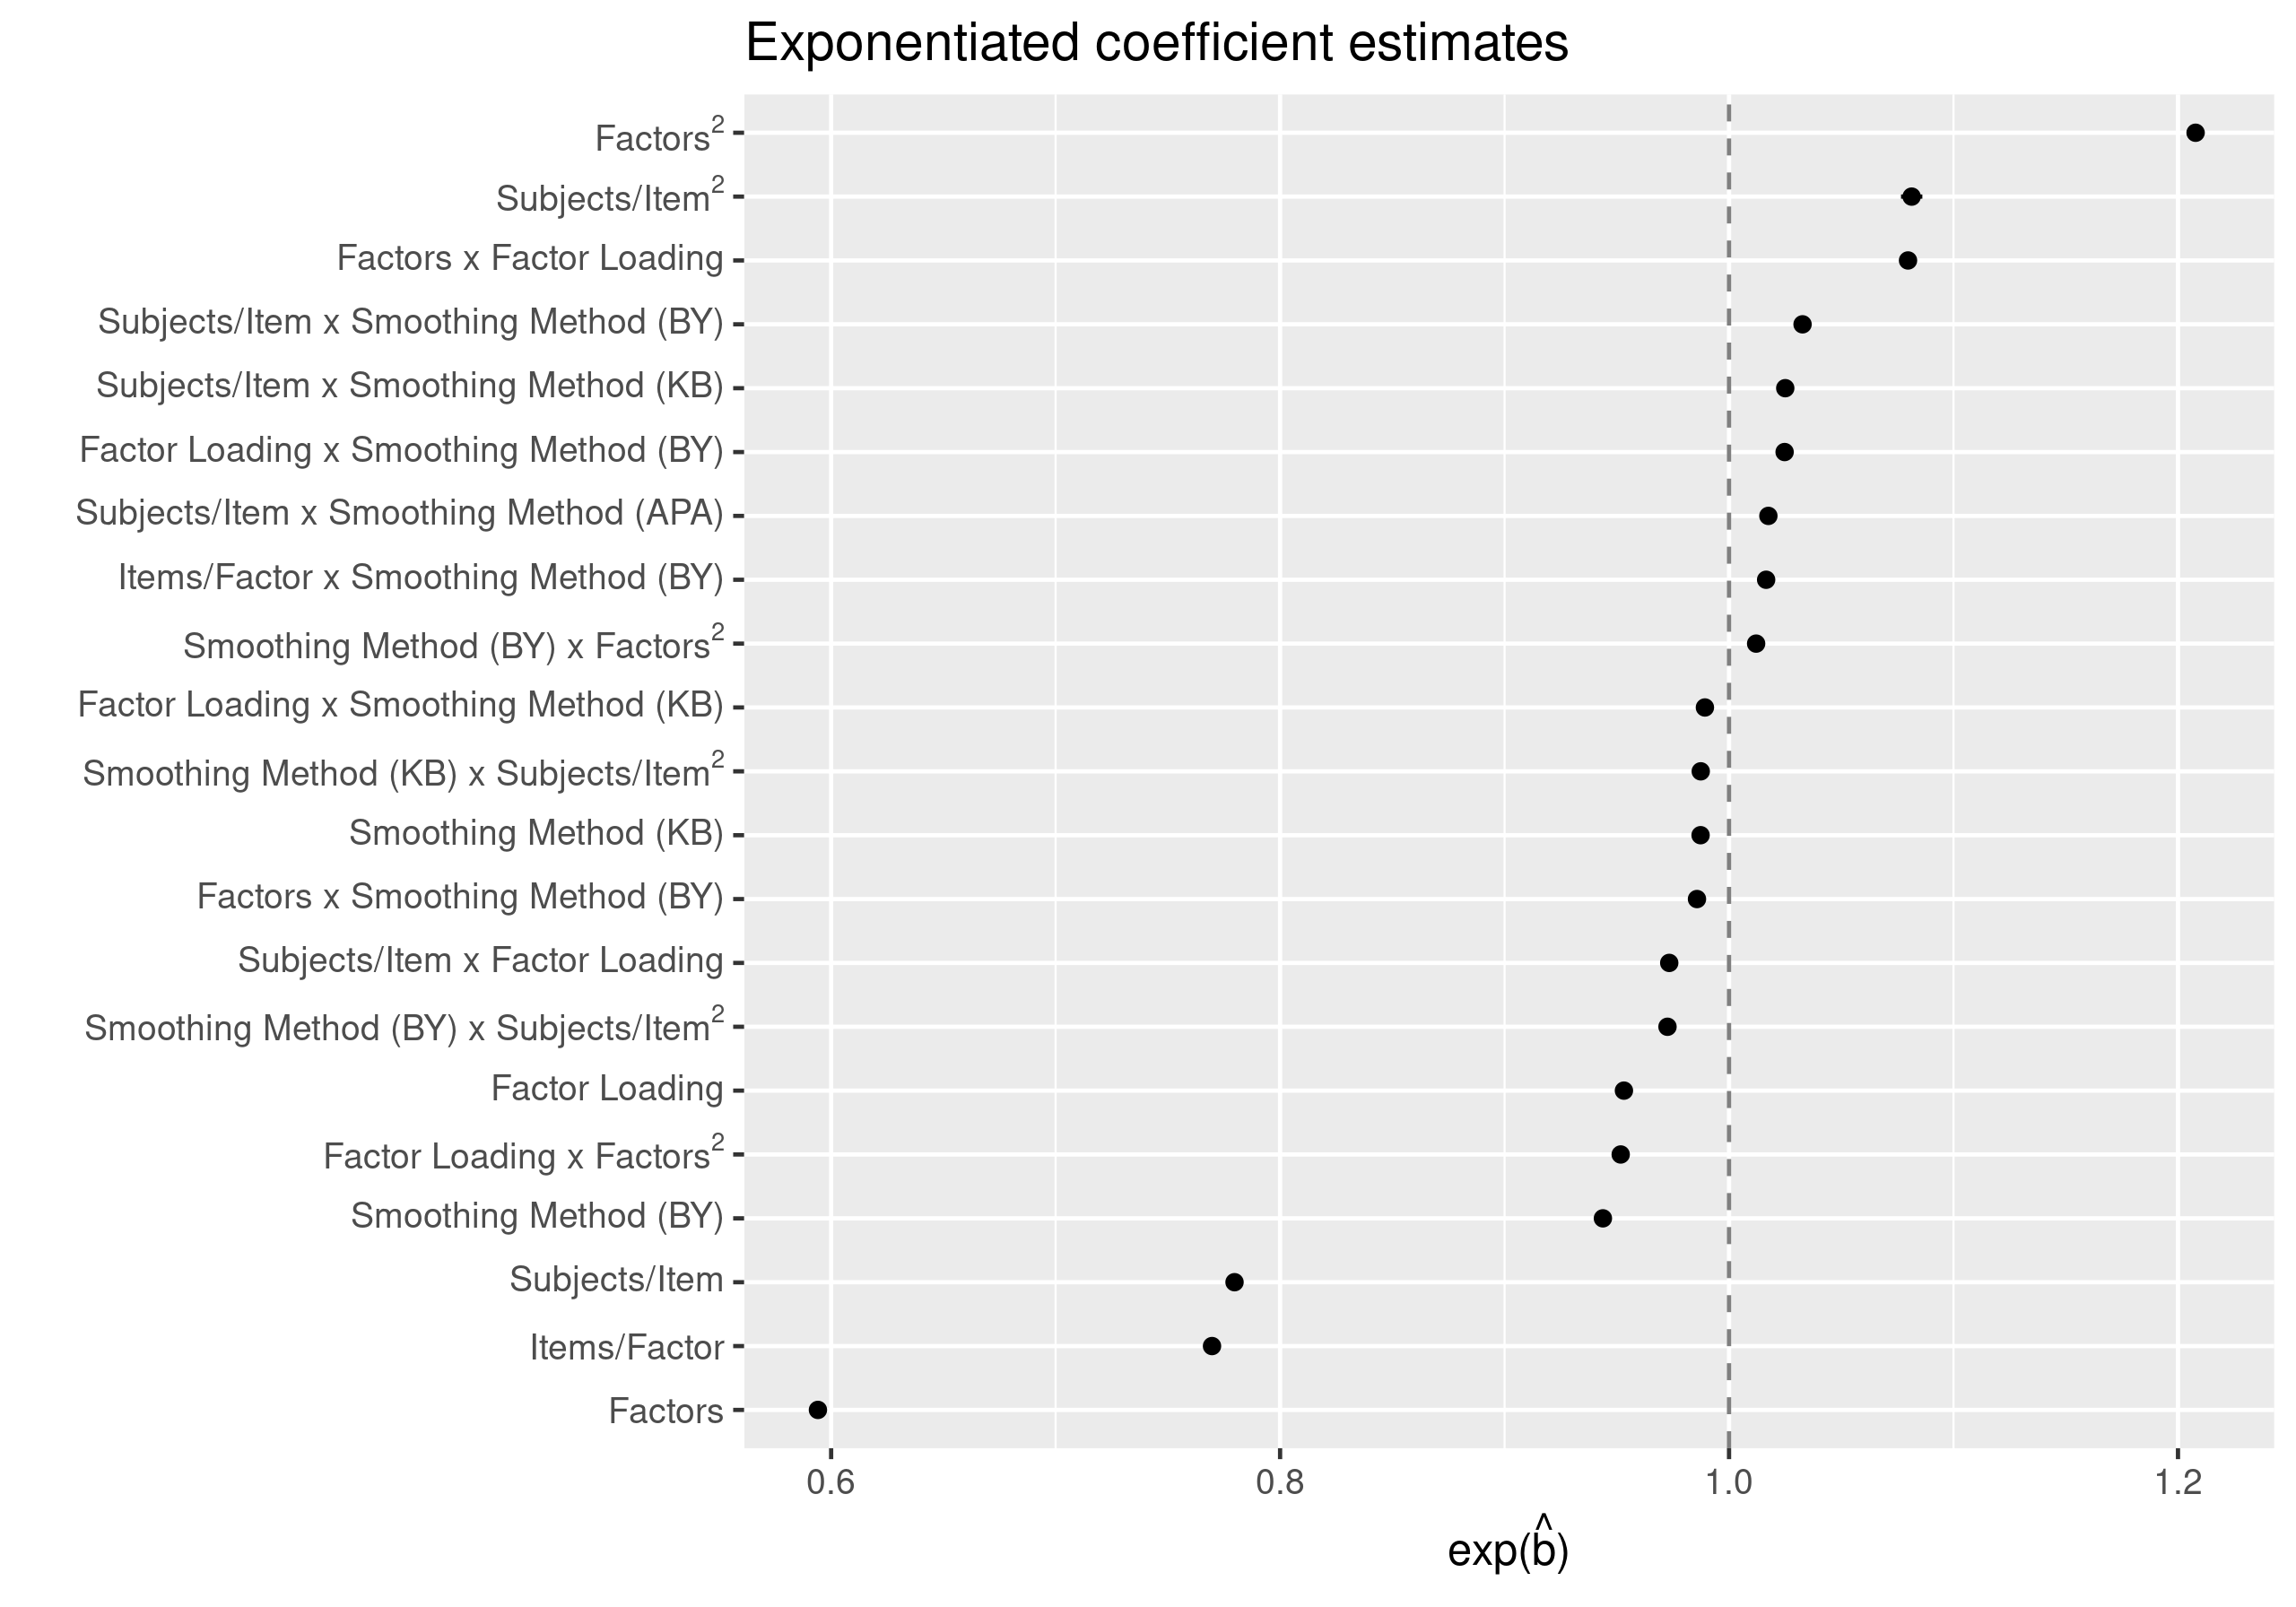
\includegraphics[width=1\linewidth]{/Volumes/GoogleDrive/My Drive/School/masters_thesis/Text/figs/RpopRsm_coefplot} 

}

\caption{Exponentiated coefficient estimates for the linear mixed effects model using $\log[\mathrm{D}_{\mathrm{s}}(\mathbf{R}_{\textrm{Sm}}, \mathbf{R}_{\textrm{Pop}})]$ as the dependent variable and estimating a random intercept for each indefinite correlation matrix. The Higham (2002), Bentler-Yuan (2011) and Knol-Berger (1991) algorithms are denoted as APA, BY, and KB, respectively. The effect of the condition where no smoothing was applied is subsumed within the Constant term.}\label{fig:coefplot-RpopRsm}
\end{figure}

\begin{figure}

{\centering 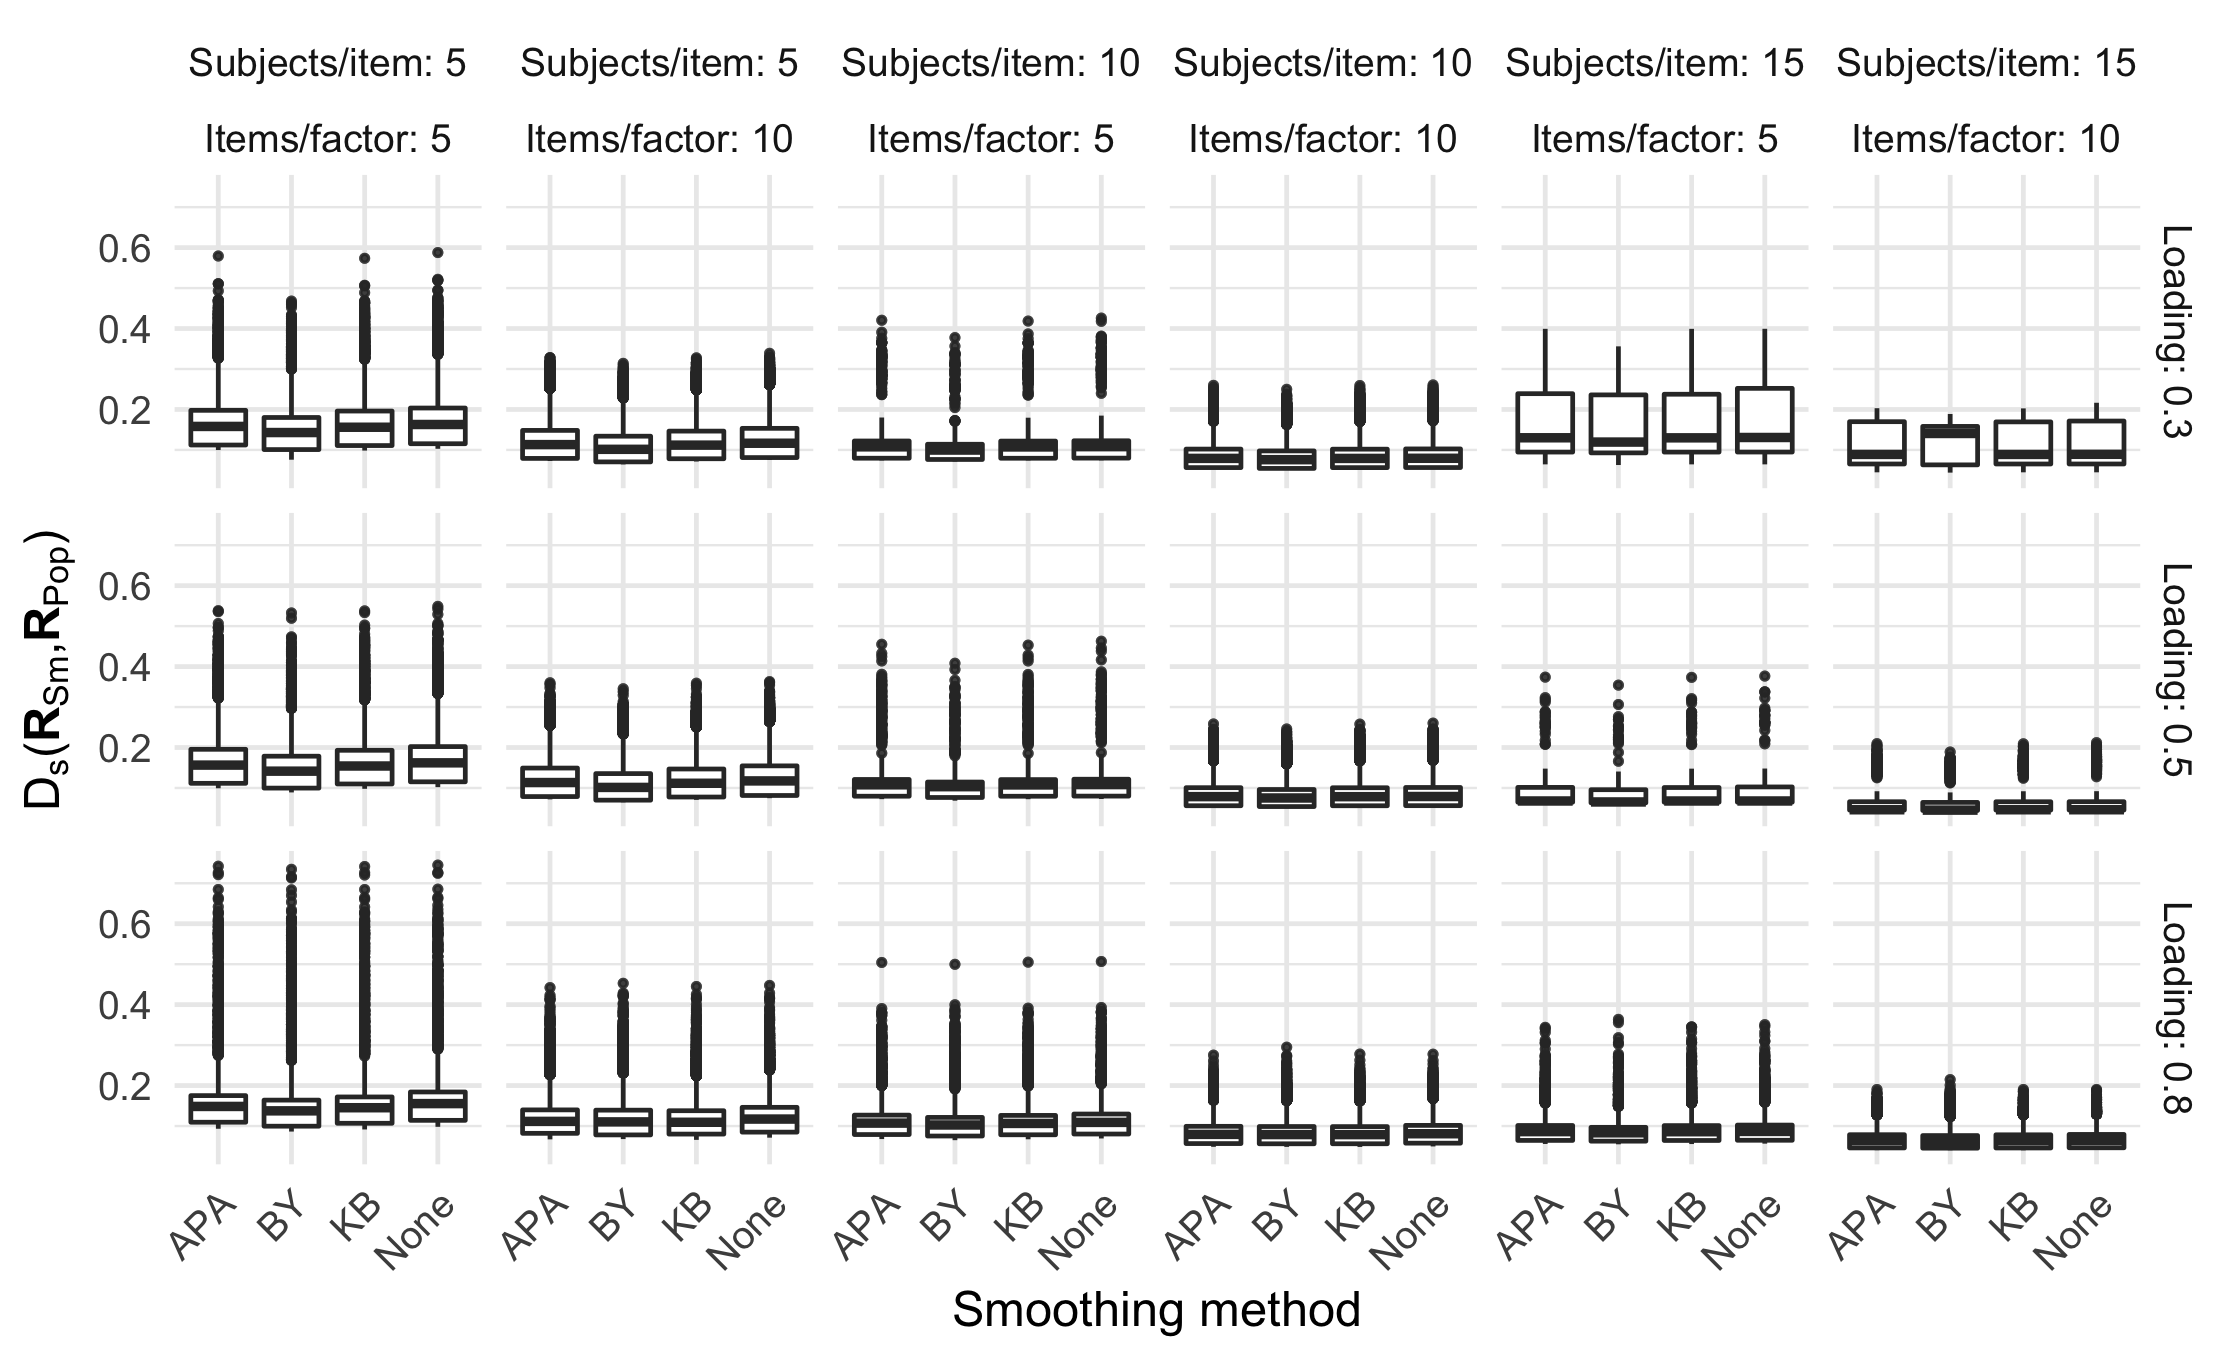
\includegraphics[width=1\linewidth]{/Volumes/GoogleDrive/My Drive/School/masters_thesis/Text/figs/distance_Rpop_Rsm} 

}

\caption{Scaled distance between the smoothed ($\mathbf{R}_{\textrm{Sm}}$) and model-implied ($\mathbf{R}_{\textrm{Pop}}$) correlation matrices for the Higham (APA; 2002), Bentler-Yuan (BY; 2011), and Knol-Berger (KB; 1991) smoothing methods and when no smoothing was applied (None).}\label{fig:distance-Rpop-Rsm}
\end{figure}

\begin{center}
\begin{longtable}{l r }
\caption{Coefficient estimates and standard errors for the linear mixed effects model using $\log[\mathrm{D}_{\mathrm{s}}(\mathbf{R}_{\textrm{Sm}}, \mathbf{R}_{\textrm{Pop}})]$ as the dependent variable and estimating a random intercept for each NPD correlation matrix.}
\label{tab:distance-mod-summary}\\
\hline
 &  \\
\hline
\endfirsthead
\hline
 &  \\
\hline
\endhead
\hline
\endfoot
\hline
\\
\endlastfoot
Constant                                       & $-2.2162 \; (0.0004)$ \\
Subjects/Item                                  & $-0.2207 \; (0.0005)$ \\
Items/Factor                                   & $-0.1638 \; (0.0004)$ \\
Factors                                        & $-0.3134 \; (0.0004)$ \\
Factor Loading                                 & $-0.0354 \; (0.0005)$ \\
Model Error                                    & $-0.0038 \; (0.0004)$ \\
Smoothing Method (APA)                         & $-0.0240 \; (0.0001)$ \\
Smoothing Method (BY)                          & $-0.0724 \; (0.0001)$ \\
Smoothing Method (KB)                          & $-0.0328 \; (0.0001)$ \\
Subjects/Item $\times$ Items/Factor            & $-0.0034 \; (0.0004)$ \\
Subjects/Item $\times$ Factors                 & $0.0104 \; (0.0004)$  \\
Subjects/Item $\times$ Factor Loading          & $0.0041 \; (0.0005)$  \\
Subjects/Item $\times$ Model Error             & $-0.0004 \; (0.0004)$ \\
Subjects/Item $\times$ Smoothing Method (APA)  & $0.0144 \; (0.0001)$  \\
Subjects/Item $\times$ Smoothing Method (BY)   & $0.0282 \; (0.0001)$  \\
Subjects/Item $\times$ Smoothing Method (KB)   & $0.0204 \; (0.0001)$  \\
Items/Factor $\times$ Factors                  & $-0.0199 \; (0.0004)$ \\
Items/Factor $\times$ Factor Loading           & $-0.0028 \; (0.0004)$ \\
Items/Factor $\times$ Model Error              & $0.0013 \; (0.0004)$  \\
Items/Factor $\times$ Smoothing Method (APA)   & $-0.0003 \; (0.0001)$ \\
Items/Factor $\times$ Smoothing Method (BY)    & $0.0128 \; (0.0001)$  \\
Items/Factor $\times$ Smoothing Method (KB)    & $0.0001 \; (0.0001)$  \\
Factors $\times$ Factor Loading                & $0.0229 \; (0.0004)$  \\
Factors $\times$ Model Error                   & $0.0007 \; (0.0004)$  \\
Factors $\times$ Smoothing Method (APA)        & $0.0016 \; (0.0001)$  \\
Factors $\times$ Smoothing Method (BY)         & $-0.0046 \; (0.0001)$ \\
Factors $\times$ Smoothing Method (KB)         & $-0.0001 \; (0.0001)$ \\
Factor Loading $\times$ Model Error            & $0.0060 \; (0.0004)$  \\
Factor Loading $\times$ Smoothing Method (APA) & $-0.0068 \; (0.0001)$ \\
Factor Loading $\times$ Smoothing Method (BY)  & $0.0193 \; (0.0001)$  \\
Factor Loading $\times$ Smoothing Method (KB)  & $-0.0092 \; (0.0001)$ \\
Model Error $\times$ Smoothing Method (APA)    & $-0.0022 \; (0.0001)$ \\
Model Error $\times$ Smoothing Method (BY)     & $0.0011 \; (0.0001)$  \\
Model Error $\times$ Smoothing Method (KB)     & $-0.0032 \; (0.0001)$ \\
\hline
AIC                                            & -1808572.2960         \\
BIC                                            & -1808172.0800         \\
Log Likelihood                                 & 904322.1480           \\
Num. obs.                                      & 497381                \\
Num. groups: id                                & 124346                \\
Var: id (Intercept)                            & 0.0175                \\
Var: Residual                                  & 0.0004                \\
\end{longtable}
\end{center}

\hypertarget{recovery-of-factor-loadings}{%
\subsection{Recovery of factor loadings}\label{recovery-of-factor-loadings}}

I next analyzed the results in terms of factor loading recovery. In particular, I sought to determine whether factor analysis of smoothed matrices led to better factor loading estimates than unsmoothed matrices, and if particular smoothing methods led to better factor loading estimates than others. I was also interested in whether the interactions between smoothing methods and the other variables (e.g., number of items per factor, number of subjects per item, factor analysis method, etc.) affected the relative smoothing algorithm performance in terms of factor loading estimation. For the purposes of these analyses, I evaluated factor loading recovery using the root-mean-square error (RMSE) between the estimated and population factor loadings for the major factors. Given a matrix of estimated major factor loadings \(\hat{\mathbf{\Lambda}} = \{ \hat{\lambda}_{ij} \}_{p \times m}\), and the corresponding matrix of population major factor loadings, \(\mathbf{\Lambda} = \{ \lambda_{ij} \}_{p \times m}\),
\begin{equation}
\textrm{RMSE}(\mathbf{\Lambda}, \hat{\mathbf{\Lambda}}) = \sqrt{\sum_{i = 1}^{p} \sum_{j = 1}^{m} \frac{(\lambda_{ij} - \hat{\lambda}_{ij})^2}{pm}}.
\label{eq:rmse}
\end{equation}

To determine which smoothing method resulted in the best factor loading estimates, I calculated the \(\textrm{RMSE}(\mathbf{\Lambda}, \hat{\mathbf{\Lambda}})\) for each pair of estimated and population factor loading matrices corresponding to the (possibly) smoothed indefinite tetrachoric correlation matrices. Relatively small \(\textrm{RMSE}(\mathbf{\Lambda}, \hat{\mathbf{\Lambda}})\) values indicated that the estimated factor loading matrices were more similar to their corresponding population factor loading matrices, whereas larger \(\textrm{RMSE}(\mathbf{\Lambda}, \hat{\mathbf{\Lambda}})\) values indicated poorly-estimated factor loading matrices. As in the previous section, the four cases where the Higham (2002) algorithm did not converge were not included in my analyses. Furthermore, cases where PA failed to converge were also not included. In total, there were 2,714 cases where the PA algorithm did not converge (convergence rate = 99.5\%) and only four cases where the ML algorithm did not converge (convergence rate \textgreater{} 99.9\%). For the 1,489,425 cases remaining, factor analysis of the Bentler-Yuan (2011) smoothed matrices resulted in the lowest mean \(\textrm{RMSE}(\mathbf{\Lambda}, \hat{\mathbf{\Lambda}})\) (\emph{M} = 0.133, \emph{SD} = 0.092) whereas the smoothed matrices produced by the Higham (2002; \emph{M} = 0.135, \emph{SD} = 0.097) and Knol-Berger (1991; \emph{M} = 0.135, \emph{SD} = 0.097) algorithms led to slightly higher mean \(\textrm{RMSE}(\mathbf{\Lambda}, \hat{\mathbf{\Lambda}})\) values. Factor analyzing unsmoothed indefinite tetrachoric correlation matrices led to the highest mean \(\textrm{RMSE}(\mathbf{\Lambda}, \hat{\mathbf{\Lambda}})\) (\emph{M} = 0.137, \emph{SD} = 0.103).

To obtain estimates of effects, I fit a linear mixed-effects model regressing \(\log \textrm{RMSE}(\mathbf{\Lambda}, \hat{\mathbf{\Lambda}})\) on number of subjects per item, number of items per factor, number of factors, factor loading, model error, smoothing algorithm (Higham, Bentler-Yuan, Knol-Berger, or no smoothing), factor analysis method (PA, OLS, or ML), all two-way interactions between these variables, and a random intercept estimated for every unique indefinite correlation matrix.\footnote{All numeric predictors were scaled to have a mean of zero and variance of one prior to analysis. Diagnostic plots can be found in Appendix A.} The estimated (exponentiated) fixed-effect coefficients are shown in Figure \ref{fig:coefplot-loading-recovery}. A full summary table including (untransformed) coefficient estimates and standard errors appears in Table \ref{tab:loading-mod-summary}.

Figure \ref{fig:coefplot-loading-recovery} shows that only a few variables had non-negligible effects on factor loading recovery. None of the effects of primary interest to this study---the main effects or two-way interactions involving the smoothing methods---were large enough to hold much practical significance. For instance, the results indicated that not applying smoothing to an indefinite tetrachoric correlation matrix prior to factor analysis led to the worst factor loading estimates among the four smoothing methods. However, this effect represented only a minute improvement in \(\textrm{RMSE}(\mathbf{\Lambda}, \hat{\mathbf{\Lambda}})\) for smoothed compared to unsmoothed indefinite tetrachoric correlation matrices (see Figure \ref{fig:coefplot-loading-recovery} and Table \ref{tab:loading-mod-summary}).

Although none of the primary effects of interest to this study were large, there were some estimated effects that, although ancillary for this study, were large enough to warrant mention. In particular, there were moderate, positive effects for ML (\(b = 0.116\), \emph{SE} = 0.0004, \(e^{0.116} = 1.123\)) and the interactions between ML and factor loading (\(b = 0.204\), \emph{SE} = 0.0002, \(e^{0.204} = 1.226\)), ML and subjects per item (\(b = 0.107\), \emph{SE} = 0.0002, \(e^{0.107} = 1.113\)), and ML and items per factor (\(b = 0.082\), \emph{SE} = 0.0002, \(e^{0.082} = 1.085\)). There was also a positive estimated effect for model error (\(b = 0.104\), \emph{SE} = 0.0005, \(e^{0.104} = 1.11\)). These results suggest that both the use of ML factor analysis (compared with PA or OLS) and higher levels of model approximation error led to worse factor loading recovery. Moreover, factor loading estimates for ML were not improved as much by increasing factor loadings, subjects per item, or items per factor (which were associated with negative effects) compared to PA or OLS. To illustrate this interaction, the effects of factor analysis method, factor loading, and number of subject per item are shown in Figure \ref{fig:fa-method-boxplots}, which contains box plots of \(\textrm{RMSE}(\mathbf{\Lambda}, \hat{\mathbf{\Lambda}})\) for each combination of these variables. This figure shows that ML often led to the lowest \(\textrm{RMSE}(\mathbf{\Lambda}, \hat{\mathbf{\Lambda}})\) values in conditions with small factor loadings but did not improve as much as OLS or PA as factor loadings increased. Similar effects can be seen for the number of subjects per item; although \(\textrm{RMSE}(\mathbf{\Lambda}, \hat{\mathbf{\Lambda}})\) values generally decreased as number of subjects per item increased for all factor analysis methods, ML seemed to benefit least.\footnote{Number of items per factor was not included in Figure \ref{fig:fa-method-boxplots} because the differences in \(\textrm{RMSE}(\mathbf{\Lambda}, \hat{\mathbf{\Lambda}})\) across levels of the condition were too small to be clearly seen.} These results should be interpreted carefully, however, because ML factor analysis when no smoothing was applied was (by necessity) conducted on Pearson correlation matrices whereas the other factor analysis algorithms were applied to the indefinite tetrachoric correlation matrices in the no smoothing condition.

There were also large, negative effects for the variables that should be expected to related to improved factor loading recovery, namely, factor loading (\(b = -0.438\), \emph{SE} = 0.0006, \(e^{-0.438} = 0.645\)), subjects per item (\(b = -0.189\), \emph{SE} = 0.0007, \(e^{-0.189} = 0.828\)), and items per factor (\(b = -0.175\), \emph{SE} = 0.0005, \(e^{-0.175} = 0.839\)). There was also a relatively large and seemingly anomalous negative effect for number of factors (\(b = -0.255\), \emph{SE} = 0.0005, \(e^{-0.255} = 0.775\)). On its face, this effect seems to suggest that data generated from models with large numbers of major factors led to better factor loading recovery. However, this effect is most likely due to the fact that, whereas number of items per factor and number of subjects per item were fully-crossed with (orthogonal to) number of factors, the total sample size and number of items for each data set were confounded with number of factors. In other words, conditions with larger numbers of factors tended to include more items in total, and therefore also tended to have larger sample sizes despite having the same numbers of indicators (items) per factor and numbers of subjects per indicator. The strong relationship between \(\log \textrm{RMSE}(\mathbf{\Lambda}, \hat{\mathbf{\Lambda}})\) and total sample size can be clearly seen in Figure \ref{fig:RMSE-sample-size}, which shows that \(\log \textrm{RMSE}(\mathbf{\Lambda}, \hat{\mathbf{\Lambda}})\) decreased as sample size increased. Therefore, it seems reasonable to conclude that the effect of number of factors can be better understood as being related to the total number of items and subjects in a data set. Similarly, the negative interaction between number of factors and ML (\(b = -0.090\), \emph{SE} = 0.0002, \(e^{-0.090} = 0.914\)) might be interpreted as an interaction between total number of items or subjects and ML. In summary, the results of the simulation study indicated that there was no meaningful advantage of using any smoothing algorithm over any other. Moreover, there was no large advantage (in terms of \(\textrm{RMSE}(\mathbf{\Lambda}, \hat{\mathbf{\Lambda}})\)) to smoothing indefinite tetrachoric correlation matrices prior to conducting exploratory factor analysis.

\begin{figure}

{\centering 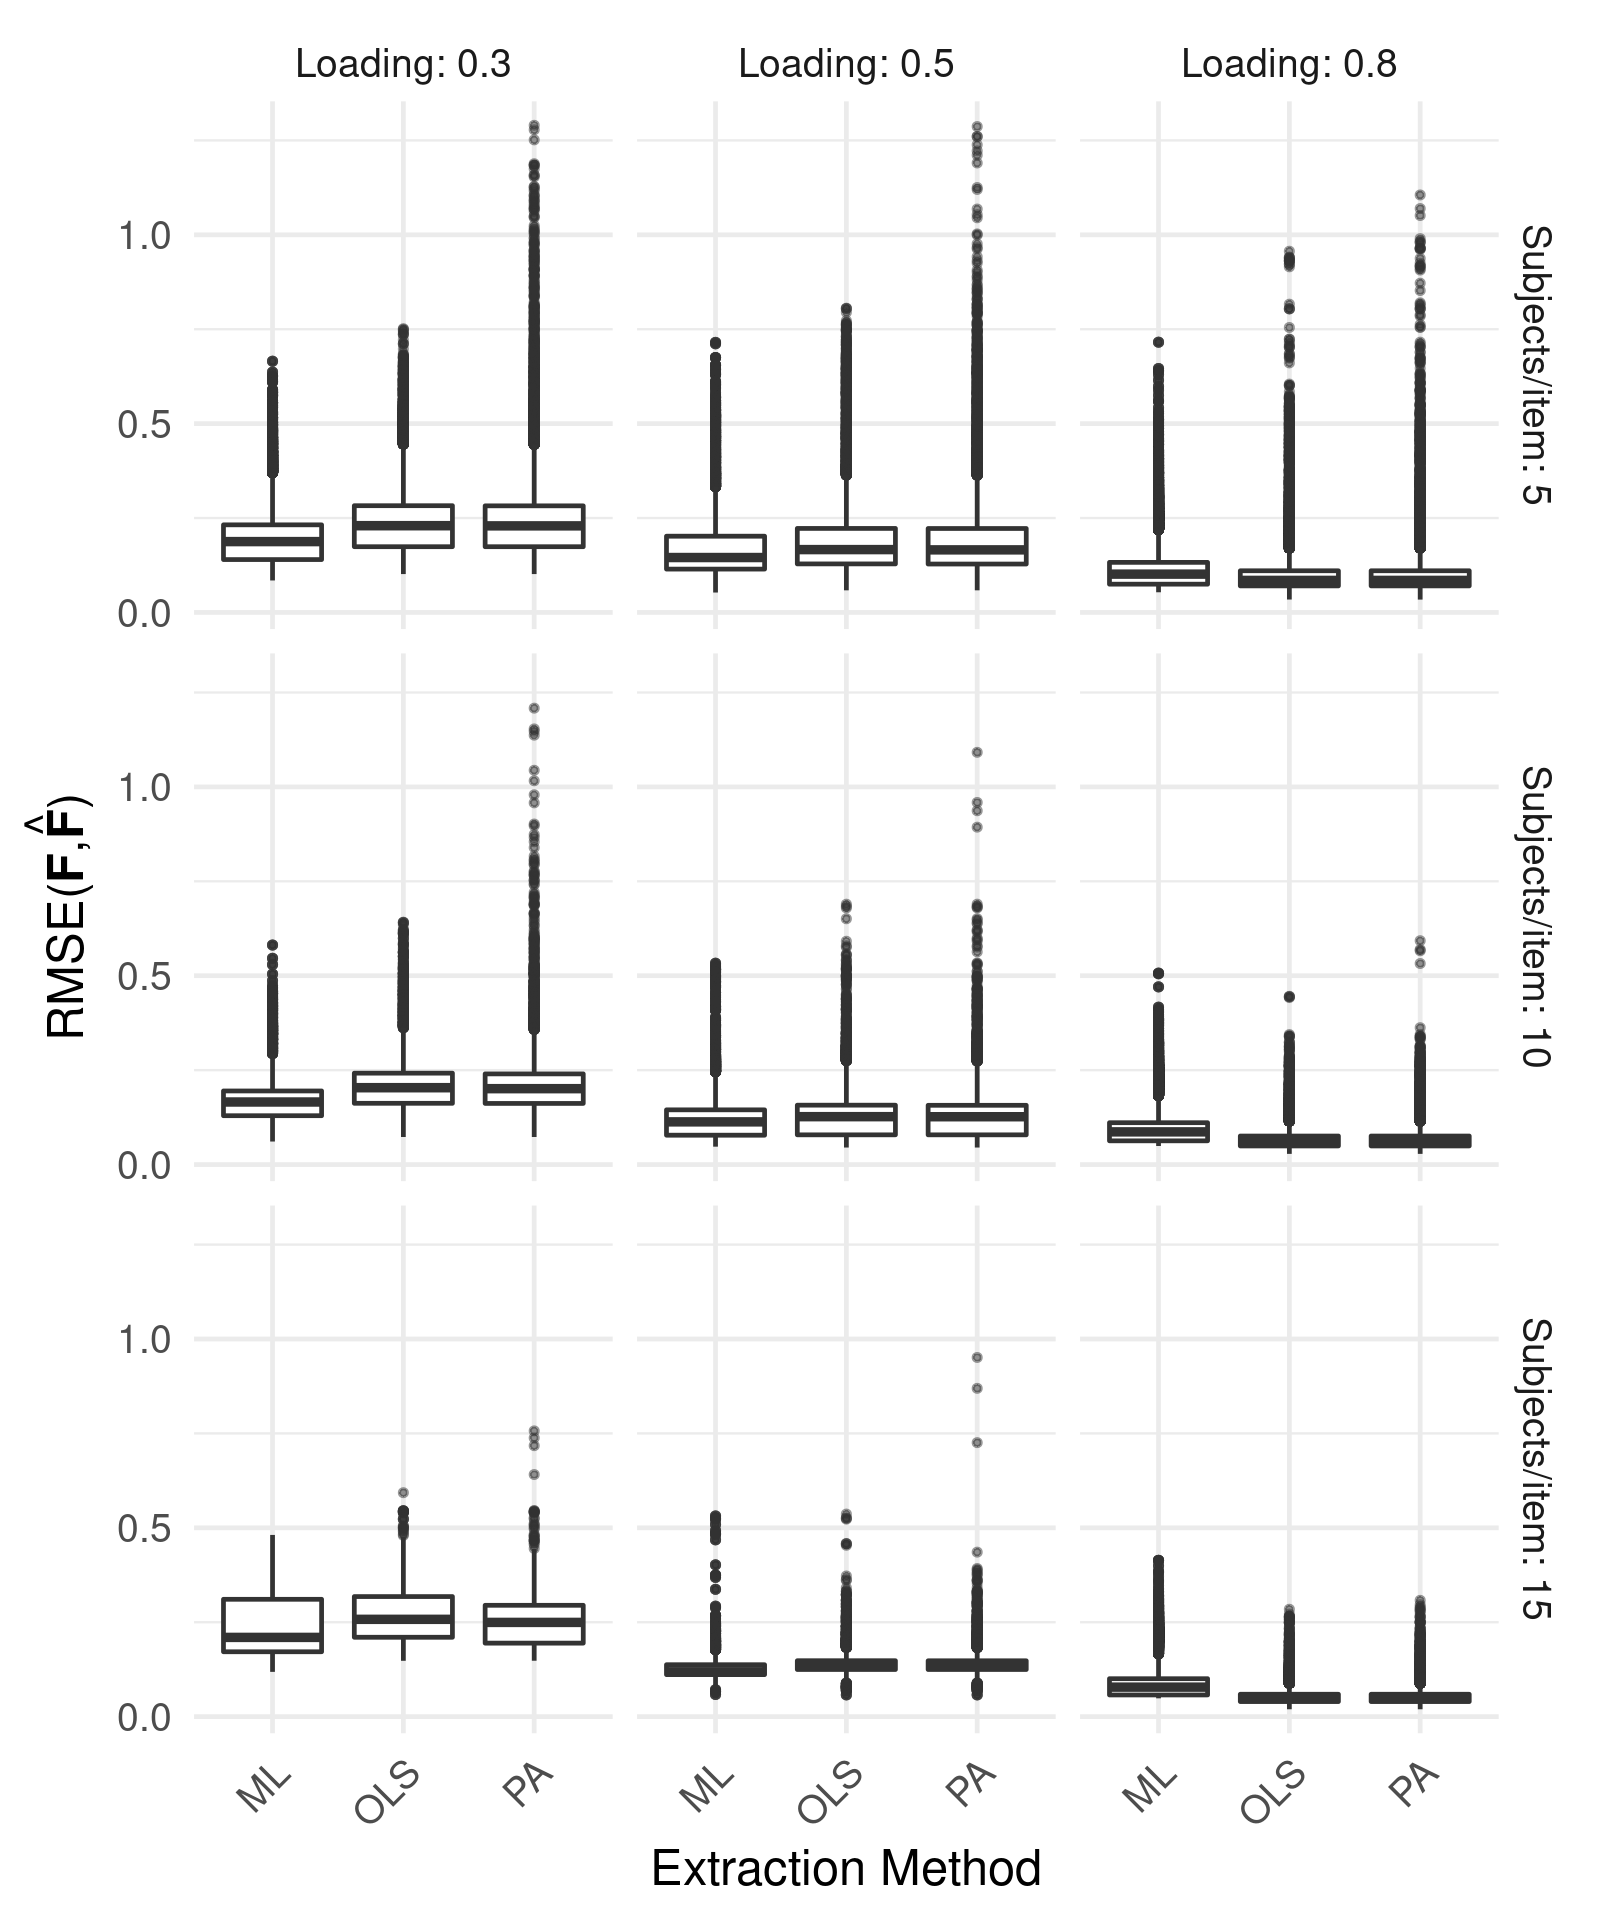
\includegraphics[width=5in]{/Volumes/GoogleDrive/My Drive/School/masters_thesis/Text/figs/fa_method_boxplots} 

}

\caption{Box plots of $\textrm{RMSE}(\mathbf{\Lambda}, \hat{\mathbf{\Lambda}})$ for all combinations of factor analysis method, factor loading, and number of subjects per item. The three factor analysis methods (ordinary least squares, maximum likelihood, and principal axes) are denoted by OLS, ML, and PA, respectively.}\label{fig:fa-method-boxplots}
\end{figure}

\begin{figure}

{\centering 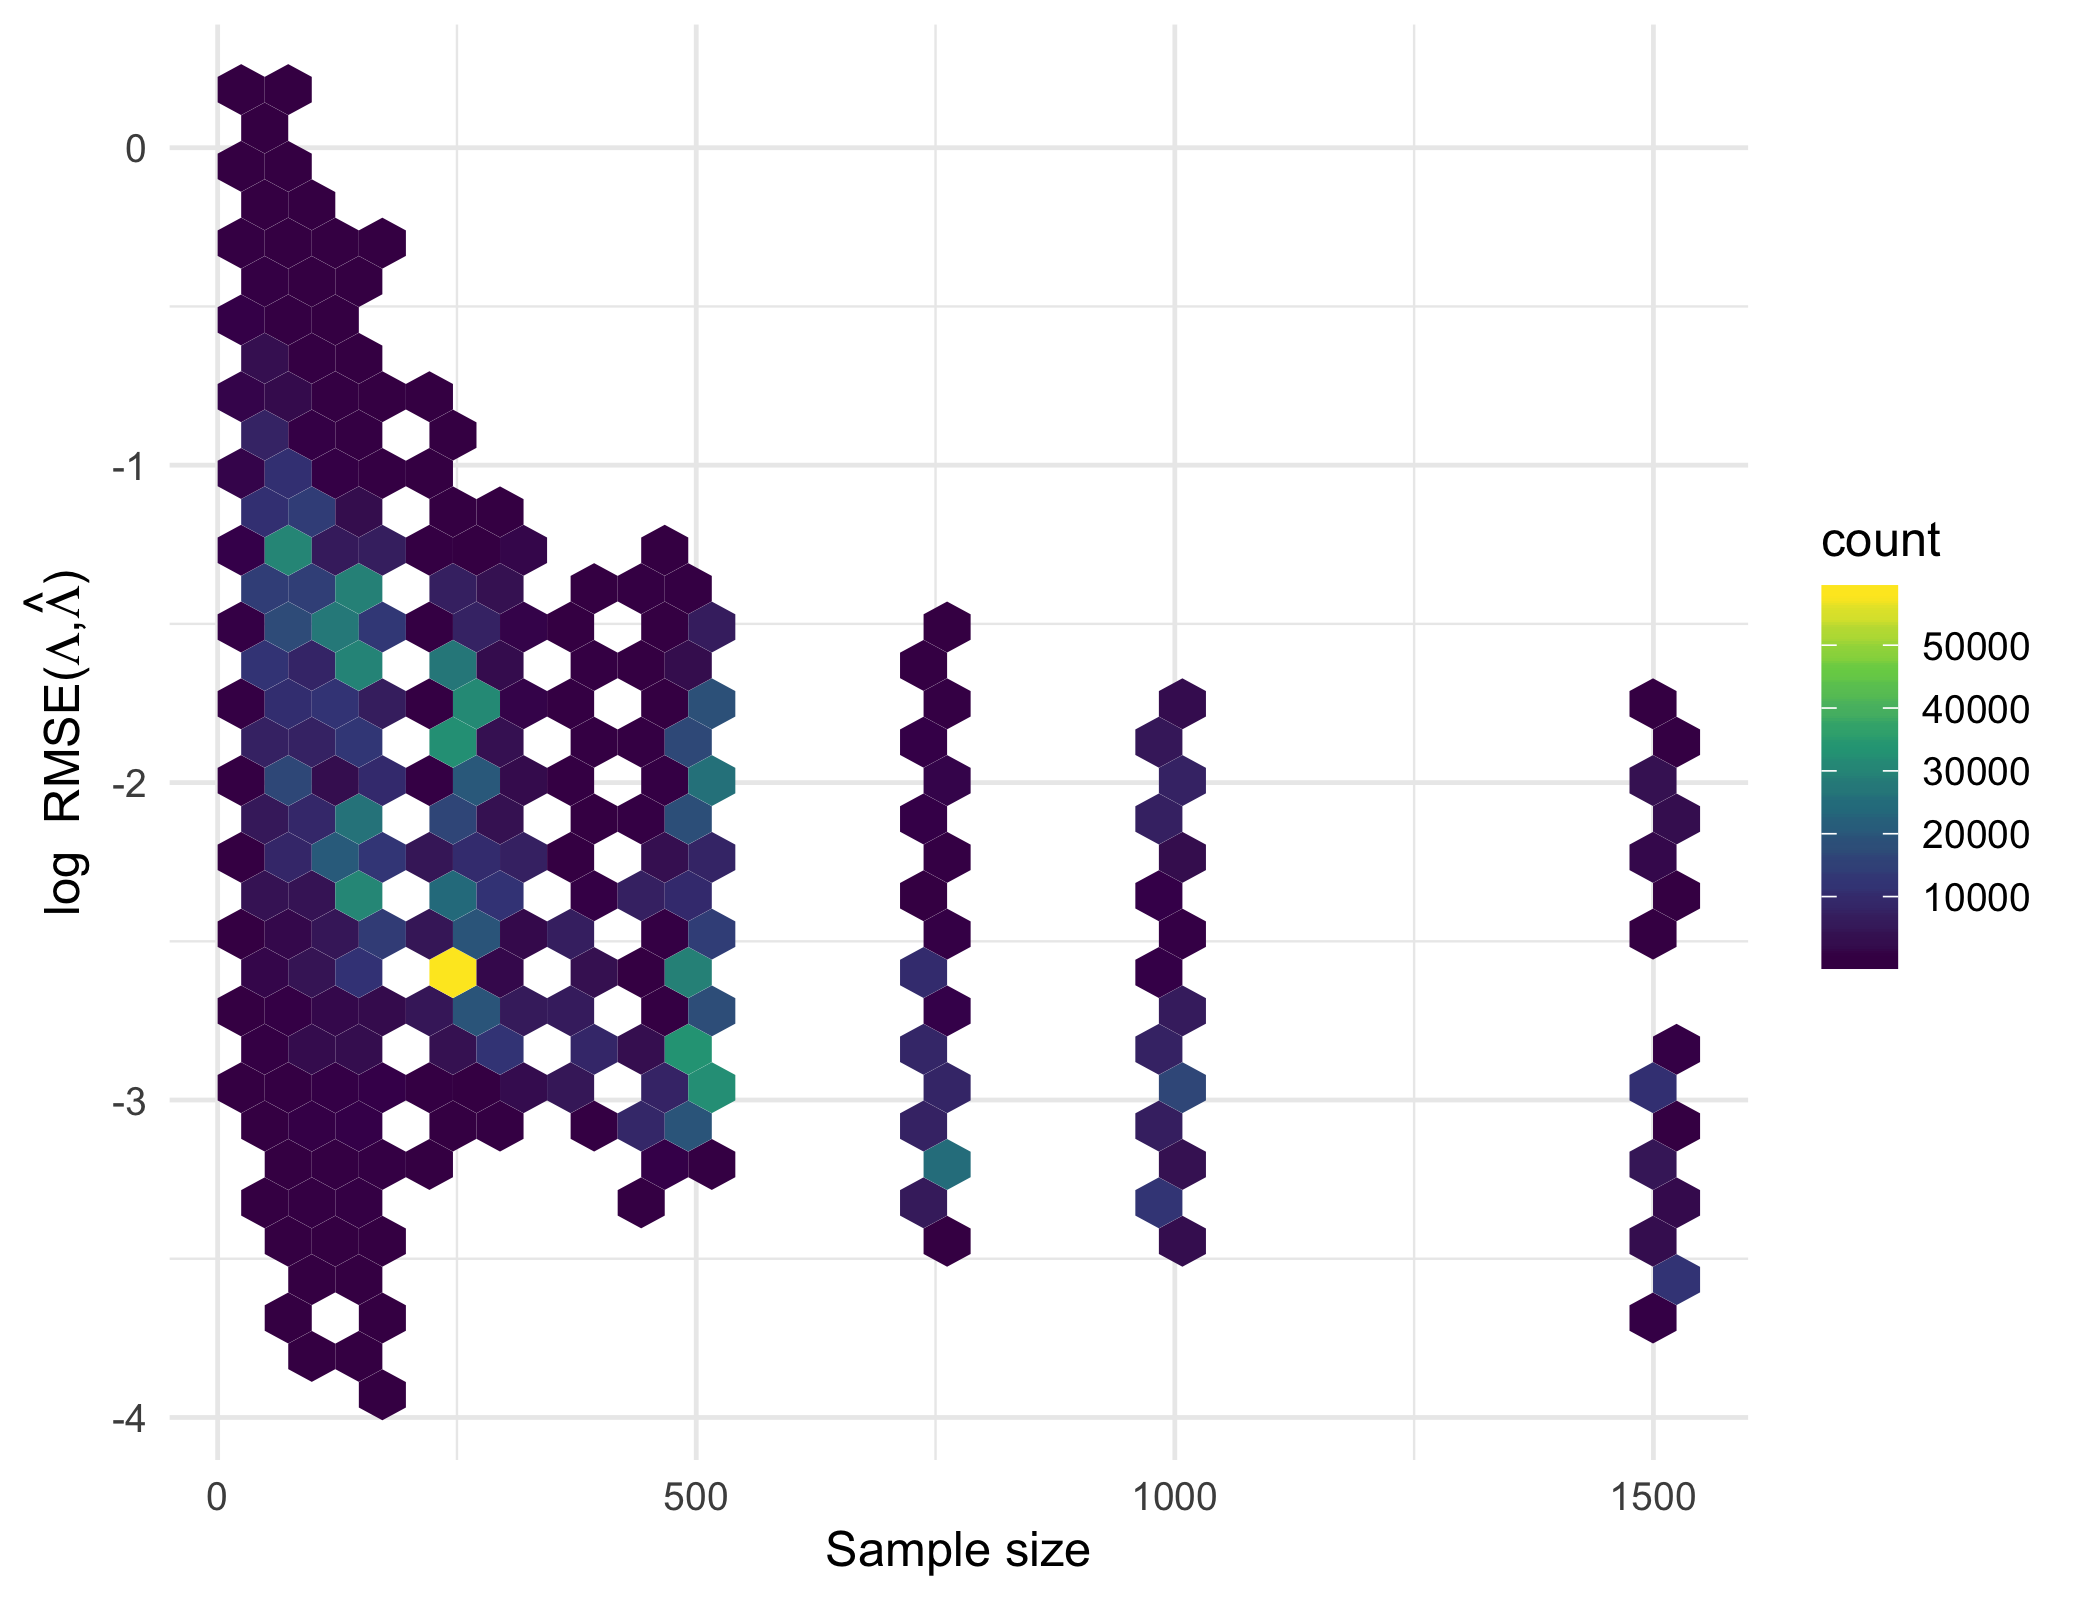
\includegraphics[width=6.5in]{/Volumes/GoogleDrive/My Drive/School/masters_thesis/Text/figs/rmse_sample_size} 

}

\caption{Log root-mean-square error (RMSE) between the true and estimated factor loading matrices as a function of sample size. Due to the large number of data points, hexagonal bins were used to group observations with the density of each hexagon represented by its color.}\label{fig:RMSE-sample-size}
\end{figure}

\begin{figure}

{\centering 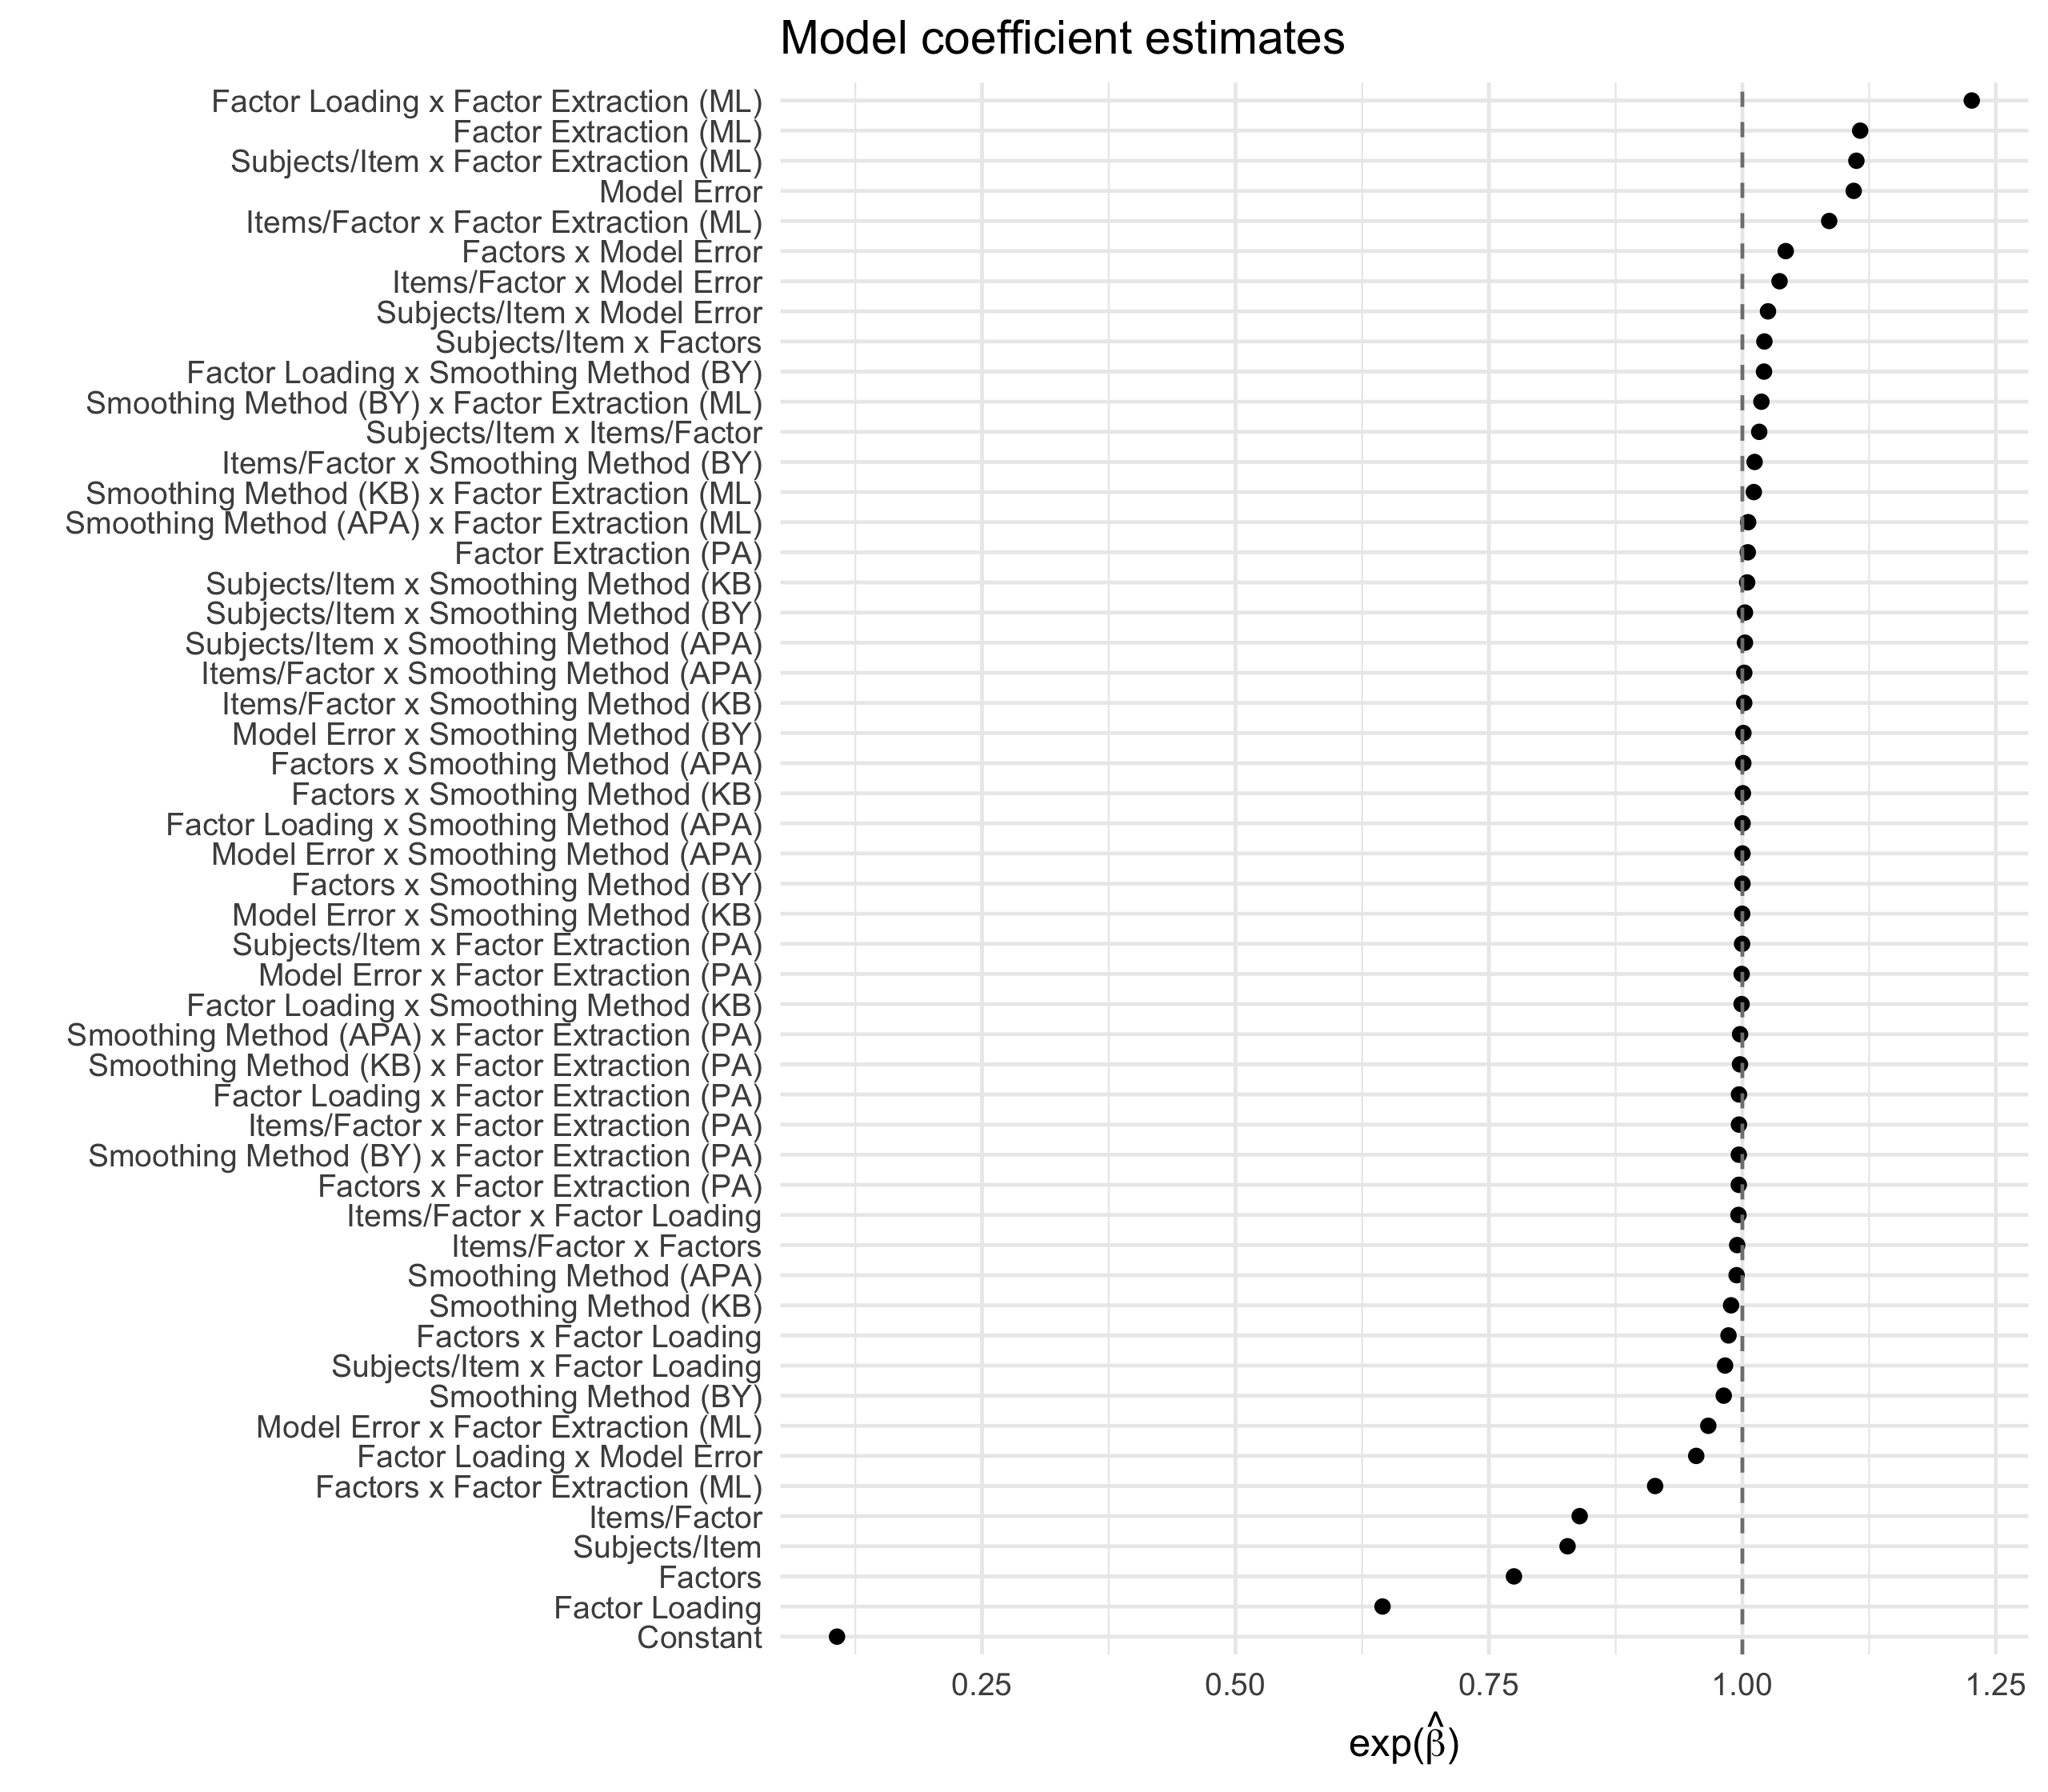
\includegraphics[width=1\linewidth]{/Volumes/GoogleDrive/My Drive/School/masters_thesis/Text/figs/loadings_coefplot} 

}

\caption{Exponentiated coefficient estimates for the linear mixed effects model using $\log[\textrm{RMSE}(\mathbf{\Lambda}, \hat{\mathbf{\Lambda}})]$ as the dependent variable and estimating a random intercept for each indefinite correlation matrix. The Higham (2002), Bentler-Yuan (2011) and Knol-Berger (1991) algorithms are denoted as APA, BY, and KB, respectively. Maximum likelihood factor analysis is denoted by ML and principal axis factor analysis is denoted by PA. The effects of no smoothing and ordinary least squares factor analysis are subsumed within the Constant term.}\label{fig:coefplot-loading-recovery}
\end{figure}

\begin{center}
\begin{longtable}{l r }
\caption{Coefficient estimates and standard errors for the linear mixed effects model using $\log[\textrm{RMSE}(\mathbf{\Lambda}, \hat{\mathbf{\Lambda}})]$ as the dependent variable and estimating a random intercept for each NPD correlation matrix.}
\label{tab:loading-mod-summary}\\
\hline
 &  \\
\hline
\endfirsthead
\hline
 &  \\
\hline
\endhead
\hline
\endfoot
\hline
\\
\endlastfoot
Constant                                               & $-2.2351 \; (0.0007)$ \\
Subjects/Item                                          & $-0.1893 \; (0.0007)$ \\
Items/Factor                                           & $-0.1749 \; (0.0005)$ \\
Factors                                                & $-0.2553 \; (0.0005)$ \\
Factor Loading                                         & $-0.4384 \; (0.0006)$ \\
Model Error                                            & $0.1042 \; (0.0005)$  \\
Smoothing Method (APA)                                 & $-0.0057 \; (0.0004)$ \\
Smoothing Method (BY)                                  & $-0.0185 \; (0.0004)$ \\
Smoothing Method (KB)                                  & $-0.0112 \; (0.0004)$ \\
Factor Extraction (ML)                                 & $0.1099 \; (0.0004)$  \\
Factor Extraction (PA)                                 & $0.0053 \; (0.0004)$  \\
Subjects/Item $\times$ Items/Factor                    & $0.0165 \; (0.0006)$  \\
Subjects/Item $\times$ Factors                         & $0.0215 \; (0.0006)$  \\
Subjects/Item $\times$ Factor Loading                  & $-0.0172 \; (0.0007)$ \\
Subjects/Item $\times$ Model Error                     & $0.0250 \; (0.0006)$  \\
Subjects/Item $\times$ Smoothing Method (APA)          & $0.0026 \; (0.0002)$  \\
Subjects/Item $\times$ Smoothing Method (BY)           & $0.0026 \; (0.0002)$  \\
Subjects/Item $\times$ Smoothing Method (KB)           & $0.0047 \; (0.0002)$  \\
Subjects/Item $\times$ Factor Extraction (ML)          & $0.1066 \; (0.0002)$  \\
Subjects/Item $\times$ Factor Extraction (PA)          & $-0.0003 \; (0.0002)$ \\
Items/Factor $\times$ Factors                          & $-0.0051 \; (0.0005)$ \\
Items/Factor $\times$ Factor Loading                   & $-0.0039 \; (0.0006)$ \\
Items/Factor $\times$ Model Error                      & $0.0360 \; (0.0005)$  \\
Items/Factor $\times$ Smoothing Method (APA)           & $0.0019 \; (0.0002)$  \\
Items/Factor $\times$ Smoothing Method (BY)            & $0.0120 \; (0.0002)$  \\
Items/Factor $\times$ Smoothing Method (KB)            & $0.0018 \; (0.0002)$  \\
Items/Factor $\times$ Factor Extraction (ML)           & $0.0822 \; (0.0002)$  \\
Items/Factor $\times$ Factor Extraction (PA)           & $-0.0034 \; (0.0002)$ \\
Factors $\times$ Factor Loading                        & $-0.0138 \; (0.0006)$ \\
Factors $\times$ Model Error                           & $0.0419 \; (0.0005)$  \\
Factors $\times$ Smoothing Method (APA)                & $0.0009 \; (0.0002)$  \\
Factors $\times$ Smoothing Method (BY)                 & $0.0001 \; (0.0002)$  \\
Factors $\times$ Smoothing Method (KB)                 & $0.0005 \; (0.0002)$  \\
Factors $\times$ Factor Extraction (ML)                & $-0.0900 \; (0.0002)$ \\
Factors $\times$ Factor Extraction (PA)                & $-0.0035 \; (0.0002)$ \\
Factor Loading $\times$ Model Error                    & $-0.0466 \; (0.0006)$ \\
Factor Loading $\times$ Smoothing Method (APA)         & $0.0002 \; (0.0002)$  \\
Factor Loading $\times$ Smoothing Method (BY)          & $0.0211 \; (0.0002)$  \\
Factor Loading $\times$ Smoothing Method (KB)          & $-0.0008 \; (0.0002)$ \\
Factor Loading $\times$ Factor Extraction (ML)         & $0.2040 \; (0.0002)$  \\
Factor Loading $\times$ Factor Extraction (PA)         & $-0.0033 \; (0.0002)$ \\
Model Error $\times$ Smoothing Method (APA)            & $0.0001 \; (0.0002)$  \\
Model Error $\times$ Smoothing Method (BY)             & $0.0010 \; (0.0002)$  \\
Model Error $\times$ Smoothing Method (KB)             & $-0.0002 \; (0.0002)$ \\
Model Error $\times$ Factor Extraction (ML)            & $-0.0342 \; (0.0002)$ \\
Model Error $\times$ Factor Extraction (PA)            & $-0.0007 \; (0.0002)$ \\
Smoothing Method (APA) $\times$ Factor Extraction (ML) & $0.0057 \; (0.0005)$  \\
Smoothing Method (BY) $\times$ Factor Extraction (ML)  & $0.0186 \; (0.0005)$  \\
Smoothing Method (KB) $\times$ Factor Extraction (ML)  & $0.0112 \; (0.0005)$  \\
Smoothing Method (APA) $\times$ Factor Extraction (PA) & $-0.0023 \; (0.0005)$ \\
Smoothing Method (BY) $\times$ Factor Extraction (PA)  & $-0.0035 \; (0.0005)$ \\
Smoothing Method (KB) $\times$ Factor Extraction (PA)  & $-0.0024 \; (0.0005)$ \\
\hline
AIC                                                    & -2414463.6688         \\
BIC                                                    & -2413804.1182         \\
Log Likelihood                                         & 1207285.8344          \\
Num. obs.                                              & 1489425               \\
Num. groups: id                                        & 124346                \\
Var: id (Intercept)                                    & 0.0316                \\
Var: Residual                                          & 0.0084                \\
\end{longtable}
\end{center}

\hypertarget{discussion}{%
\section{Discussion}\label{discussion}}

\hypertarget{interpretation-of-results}{%
\subsection{Interpretation of Results}\label{interpretation-of-results}}

The current study examined how the application of three matrix smoothing algorithms (the Higham {[}2002{]}, Bentler-Yuan {[}2011{]}, and Knol-Berger {[}1991{]} algorithms) to indefinite tetrachoric correlation matrices affected both (a) the recovery of the model-implied population correlation matrix (\(\mathbf{R}_{\textrm{Pop}}\)), and (b) the recovery of the population item factor loadings in EFA (compared to leaving the indefinite correlation matrices unsmoothed). With respect to recovery of \(\mathbf{R}_{\textrm{Pop}}\), I found that the application of any of the matrix smoothing algorithms included in the present study led to slightly better recovery of the \(\mathbf{R}_{\textrm{Pop}}\) compared to the unsmoothed, indefinite tetrachoric correlation matrix. Of the three matrix smoothing algorithms included in this study, the application of the Bentler-Yuan algorithm (2011) produced the best approximations of \(\mathbf{R}_{\textrm{Pop}}\) (on average). In particular, the Bentler-Yuan algorithm led to the best results relative to the other smoothing algorithms in conditions with low factor loadings, few items per factor, and few subjects per item. However, differences between smoothing algorithms (in terms of recovery of \(\mathbf{R}_{\textrm{Pop}}\)) were mostly so small as to be of little practical importance. With respect to the recovery of population factor loadings, I found that the particular matrix smoothing algorithm applied to an indefinite tetrachoric correlation matrix prior to EFA led to no meaningful differences in factor loading recovery. Moreover, conducting EFA on smoothed, PSD correlation matrices led to only marginally better factor loading recovery compared to conducting EFA on indefinite, unsmoothed correlation matrices.

\hypertarget{limitations-and-future-directions}{%
\subsection{Limitations and Future Directions}\label{limitations-and-future-directions}}

As with any simulation study, the present simulation design was not able to cover the full range of realistic data scenarios. For instance, the simulation design included only orthogonal population factor models and did not allow for correlated factors. Future research on this topic should investigate whether more complex correlation structures affect the performance of matrix smoothing algorithms in terms of population correlation matrix recovery and factor loading recovery. Moreover, the present studies only investigated the effects of matrix smoothing on indefinite tetrachoric correlation matrices. Further research should be done to investigate the effects of matrix smoothing on indefinite polychoric correlation matrices, as well as correlation matrices that are indefinite due to other causes. For instance, indefinite correlation matrices calculated using pairwise deletion (Wothke, 1993) or composite correlation matrices used in meta-analysis (Furlow \& Beretvas, 2005). Little is known about whether the mechanism or \enquote{cause} of indefinite correlation matrices affects their structure or how these potential differences might interact with the application of matrix smoothing algorithms.

Future research should also investigate ways to side-step the problem of indefinite tetrachoric correlation matrices. For instance, Choi, Kim, Chen, and Dannels (2011) found that polychoric correlation matrices estimated using expected a posteriori (EAP) rather than maximum-likelihood estimation led to estimates that were negatively biased but produced comparable (or smaller) RMSE values in terms of recovering the \enquote{true} correlations. It seems plausible that the slight shrinkage induced by using EAP as an estimation method would make indefinite tetrachoric or polychoric correlation matrices less common. Finally, full-information maximum likelihood (FIML; Bock \& Aitkin, 1981) can be used to estimate model parameters directly and doesn't require the estimation of a tetrachoric correlation matrix. Future research should investigate whether the use of FIML (which is computationally intensive, particularly with large models) offers any benefit, in terms of parameter recovery, when applied to data sets corresponding to indefinite tetrachoric correlation matrices.

\hypertarget{conclusion}{%
\subsection{Conclusion}\label{conclusion}}

Despite the lackluster improvement in factor loading recovery when factor analysis was conducted on smoothed rather than indefinite tetrachoric correlation matrices, the application of one of the three investigated matrix smoothing algorithms on indefinite tetrachoric correlation matrices is still recommended. None of the smoothing algorithms regularly led to worse results (in terms of factor loading recovery) compared to the conditions where the indefinite correlation matrix was left unsmoothed. Moreover, all of the smoothing algorithms investigated in this study are computationally inexpensive and are readily available as functions in R packages. For instance, the \emph{fungible} (Waller, 2019), \emph{sfsmisc} (Maechler, 2019), and \emph{Matrix} (Bates \& Maechler, 2019) packages all contain implementations of at least one of the three smoothing algorithms discussed in this article. In particular, the Knol-Berger algorithm (1991) is recommended as a smoothing algorithm that is fast, easily implemented in most programming languages, does not have convergence issues, and led to results comparable to the Bentler-Yuan and Higham algorithms.

This recommendation comes with a strong caveat; Namely, that no matrix smoothing algorithm can reasonably be considered a remedy or solution for indefinite tetrachoric correlation matrices. Instead, researchers should consider indefinite tetrachoric correlation matrices to be symptoms of larger problems (e.g., small sample sizes, bad items. etc.) and be aware that practical solutions such as gathering more data or discarding bad items are likely to lead to better results than the application of matrix smoothing algorithms. In particular, indefinite tetrachoric correlation matrices are less likely to occur when sample sizes are large relative to the number of items (see Table 1 in Debelak \& Tran, 2013, p. 70), allowing researchers to avoid the question of how to properly deal with an indefinite tetrachoric correlation matrix entirely. If collecting more data is not possible, researchers should consider removing problematic items. In short, all three investigated smoothing algorithms are reasonable choices for dealing with indefinite tetrachoric correlation matrices prior to factor analysis and seem to offer a modest benefit (in terms of factor loading recovery) compared to leaving the indefinite tetrachoric correlation matrix unsmoothed. However, the application of these algorithms should be considered to be little more than a band-aid fix that does not address the underlying issues leading to indefinite tetrachoric correlation matrices.

\newpage

\hypertarget{references}{%
\section{References}\label{references}}

\begingroup
\setlength{\parindent}{-0.5in}
\setlength{\leftskip}{0.5in}

\hypertarget{refs}{}
\leavevmode\hypertarget{ref-R-papaja}{}%
Aust, F., \& Barth, M. (2018). \emph{papaja: Create APA manuscripts with R Markdown}. Retrieved from \url{https://github.com/crsh/papaja}

\leavevmode\hypertarget{ref-banerjee2014}{}%
Banerjee, S., \& Roy, A. (2014). \emph{Linear algebra and matrix analysis for statistics}. Chapman; Hall/CRC.

\leavevmode\hypertarget{ref-R-questionr}{}%
Barnier, J., Briatte, F., \& Larmarange, J. (2018). \emph{Questionr: Functions to make surveys processing easier}. Retrieved from \url{https://CRAN.R-project.org/package=questionr}

\leavevmode\hypertarget{ref-R-Matrix}{}%
Bates, D., \& Maechler, M. (2019). \emph{Matrix: Sparse and dense matrix classes and methods}. Retrieved from \url{https://CRAN.R-project.org/package=Matrix}

\leavevmode\hypertarget{ref-R-lme4}{}%
Bates, D., Mächler, M., Bolker, B., \& Walker, S. (2015). Fitting linear mixed-effects models using lme4. \emph{Journal of Statistical Software}, \emph{67}(1), 1--48. \url{https://doi.org/10.18637/jss.v067.i01}

\leavevmode\hypertarget{ref-bentler1972}{}%
Bentler, P. (1972). A lower-bound method for the dimension-free measurement of internal consistency. \emph{Social Science Research}, \emph{1}(4), 343--357.

\leavevmode\hypertarget{ref-bentler2011}{}%
Bentler, P., \& Yuan, K.-H. (2011). Positive definiteness via off-diagonal scaling of a symmetric indefinite matrix. \emph{Psychometrika}, \emph{76}(1), 119--123.

\leavevmode\hypertarget{ref-birnbaum1968some}{}%
Birnbaum, A. L. (1968). Some latent trait models and their use in inferring an examinee's ability. \emph{Statistical Theories of Mental Test Scores}.

\leavevmode\hypertarget{ref-bock1981}{}%
Bock, R. D., \& Aitkin, M. (1981). Marginal maximum likelihood estimation of item parameters: Application of an em algorithm. \emph{Psychometrika}, \emph{46}(4), 443--459. \url{https://doi.org/10.1007/BF02293801}

\leavevmode\hypertarget{ref-bock1988}{}%
Bock, R. D., Gibbons, R., \& Muraki, E. (1988). Full-information item factor analysis. \emph{Applied Psychological Measurement}, \emph{12}(3), 261--280.

\leavevmode\hypertarget{ref-R-broom.mixed}{}%
Bolker, B., \& Robinson, D. (2019). \emph{Broom.mixed: Tidying methods for mixed models}. Retrieved from \url{https://CRAN.R-project.org/package=broom.mixed}

\leavevmode\hypertarget{ref-box1964}{}%
Box, G. E., \& Cox, D. R. (1964). An analysis of transformations. \emph{Journal of the Royal Statistical Society: Series B (Methodological)}, \emph{26}(2), 211--243.

\leavevmode\hypertarget{ref-briggs2003}{}%
Briggs, N. E., \& MacCallum, R. C. (2003). Recovery of weak common factors by maximum likelihood and ordinary least squares estimation. \emph{Multivariate Behavioral Research}, \emph{38}(1), 25--56.

\leavevmode\hypertarget{ref-brown1977mean}{}%
Brown, M. B., \& Benedetti, J. K. (1977). On the mean and variance of the tetrachoric correlation coefficient. \emph{Psychometrika}, \emph{42}(3), 347--355.

\leavevmode\hypertarget{ref-butler1992}{}%
Butler, S. M., \& Louis, T. A. (1992). Random effects models with non-parametric priors. \emph{Statistics in Medicine}, \emph{11}(14-15), 1981--2000.

\leavevmode\hypertarget{ref-carroll1957}{}%
Carroll, J. B. (1957). Biquartimin criterion for rotation to oblique simple structure in factor analysis. \emph{Science}, \emph{126}, 1114--1115. \url{https://doi.org/10.1126/science.126.3283.1114}

\leavevmode\hypertarget{ref-choi2011}{}%
Choi, J., Kim, S., Chen, J., \& Dannels, S. (2011). A comparison of maximum likelihood and Bayesian estimation for polychoric correlation using monte carlo simulation. \emph{Journal of Educational and Behavioral Statistics}, \emph{36}(4), 523--549.

\leavevmode\hypertarget{ref-comrey1962minimum}{}%
Comrey, A. L. (1962). The minimum residual method of factor analysis. \emph{Psychological Reports}, \emph{11}(1), 15--18.

\leavevmode\hypertarget{ref-CrockerAlgina}{}%
Crocker, L., \& Algina, J. (1986). \emph{Introduction to classical and modern test theory.} ERIC.

\leavevmode\hypertarget{ref-cudeck1991model}{}%
Cudeck, R., \& Henly, S. J. (1991). Model selection in covariance structures analysis and the ``problem'' of sample size: A clarification. \emph{Psychological Bulletin}, \emph{109}(3), 512.

\leavevmode\hypertarget{ref-de2013theory}{}%
de Ayala, R. J. (2013). \emph{The theory and practice of item response theory}. Guilford Publications.

\leavevmode\hypertarget{ref-debelak2013}{}%
Debelak, R., \& Tran, U. S. (2013). Principal component analysis of smoothed tetrachoric correlation matrices as a measure of dimensionality. \emph{Educational and Psychological Measurement}, \emph{73}(1), 63--77.

\leavevmode\hypertarget{ref-debelak2016}{}%
Debelak, R., \& Tran, U. S. (2016). Comparing the effects of different smoothing algorithms on the assessment of dimensionality of ordered categorical items with parallel analysis. \emph{PLOS ONE}, \emph{11}(2), 1--18. \url{https://doi.org/10.1371/journal.pone.0148143}

\leavevmode\hypertarget{ref-devlin1975robust}{}%
Devlin, S. J., Gnanadesikan, R., \& Kettenring, J. R. (1975). Robust estimation and outlier detection with correlation coefficients. \emph{Biometrika}, \emph{62}(3), 531--545.

\leavevmode\hypertarget{ref-dillon1987}{}%
Dillon, W. R., Kumar, A., \& Mulani, N. (1987). Offending estimates in covariance structure analysis: Comments on the causes of and solutions to heywood cases. \emph{Psychological Bulletin}, \emph{101}(1), 126.

\leavevmode\hypertarget{ref-divgi1979}{}%
Divgi, D. R. (1979). Calculation of the tetrachoric correlation coefficient. \emph{Psychometrika}, \emph{44}(2), 169--172. \url{https://doi.org/10.1007/BF02293968}

\leavevmode\hypertarget{ref-dong1985non}{}%
Dong, H.-K. (1985). Non-gramian and singular matrices in maximum likelihood factor analysis. \emph{Applied Psychological Measurement}, \emph{9}(4), 363--366.

\leavevmode\hypertarget{ref-dwyer1939contribution}{}%
Dwyer, P. S. (1939). The contribution of an orthogonal multiple factor solution to multiple correlation. \emph{Psychometrika}, \emph{4}(2), 163--171.

\leavevmode\hypertarget{ref-fabrigar1999evaluating}{}%
Fabrigar, L. R., Wegener, D. T., MacCallum, R. C., \& Strahan, E. J. (1999). Evaluating the use of exploratory factor analysis in psychological research. \emph{Psychological Methods}, \emph{4}(3), 272.

\leavevmode\hypertarget{ref-R-car}{}%
Fox, J., \& Weisberg, S. (2019). \emph{An R companion to applied regression} (Third). Thousand Oaks CA: Sage. Retrieved from \url{https://socialsciences.mcmaster.ca/jfox/Books/Companion/}

\leavevmode\hypertarget{ref-furlow2005}{}%
Furlow, C. F., \& Beretvas, S. N. (2005). Meta-analytic methods of pooling correlation matrices for structural equation modeling under different patterns of missing data. \emph{Psychological Methods}, \emph{10}(2), 227.

\leavevmode\hypertarget{ref-fushiki2009}{}%
Fushiki, T. (2009). Estimation of positive semidefinite correlation matrices by using convex quadratic semidefinite programming. \emph{Neural Computation}, \emph{21}(7), 2028--2048.

\leavevmode\hypertarget{ref-R-viridis}{}%
Garnier, S. (2018). \emph{Viridis: Default color maps from 'matplotlib'}. Retrieved from \url{https://CRAN.R-project.org/package=viridis}

\leavevmode\hypertarget{ref-R-arm}{}%
Gelman, A., \& Su, Y.-S. (2018). \emph{Arm: Data analysis using regression and multilevel/hierarchical models}. Retrieved from \url{https://CRAN.R-project.org/package=arm}

\leavevmode\hypertarget{ref-hair2018}{}%
Hair, J. F., Black, W. C., Babin, B. J., \& Anderson, R. E. (2018). \emph{Multivariate data analysis}. Cengage.

\leavevmode\hypertarget{ref-R-purrr}{}%
Henry, L., \& Wickham, H. (2019). \emph{Purrr: Functional programming tools}. Retrieved from \url{https://CRAN.R-project.org/package=purrr}

\leavevmode\hypertarget{ref-higham2002}{}%
Higham, N. J. (2002). Computing the nearest correlation matrix---a problem from finance. \emph{IMA Journal of Numerical Analysis}, \emph{22}(3), 329--343.

\leavevmode\hypertarget{ref-hong1999}{}%
Hong, S. (1999). Generating correlation matrices with model error for simulation studies in factor analysis: A combination of the Tucker-Koopman-Linn model and Wijsman's algorithm. \emph{Behavior Research Methods, Instruments, \& Computers}, \emph{31}(4), 727--730.

\leavevmode\hypertarget{ref-horn1965}{}%
Horn, J. L. (1965). A rationale and test for the number of factors in factor analysis. \emph{Psychometrika}, \emph{30}(2), 179--185.

\leavevmode\hypertarget{ref-jacqmin2007}{}%
Jacqmin-Gadda, H., Sibillot, S., Proust, C., Molina, J.-M., \& Thiébaut, R. (2007). Robustness of the linear mixed model to misspecified error distribution. \emph{Computational Statistics \& Data Analysis}, \emph{51}(10), 5142--5154.

\leavevmode\hypertarget{ref-jamshidian1998}{}%
Jamshidian, M., \& Bentler, P. M. (1998). A quasi-Newton method for minimum trace factor analysis. \emph{Journal of Statistical Computation and Simulation}, \emph{62}(1-2), 73--89.

\leavevmode\hypertarget{ref-jennrich2002}{}%
Jennrich, R. I. (2002). A simple general method for oblique rotation. \emph{Psychometrika}, \emph{67}(1), 7--19. \url{https://doi.org/10.1007/BF02294706}

\leavevmode\hypertarget{ref-knol1991}{}%
Knol, D. L., \& Berger, M. P. (1991). Empirical comparison between factor analysis and multidimensional item response models. \emph{Multivariate Behavioral Research}, \emph{26}(3), 457--477.

\leavevmode\hypertarget{ref-R-merTools}{}%
Knowles, J. E., \& Frederick, C. (2019). \emph{MerTools: Tools for analyzing mixed effect regression models}. Retrieved from \url{https://CRAN.R-project.org/package=merTools}

\leavevmode\hypertarget{ref-robustlmm}{}%
Koller, M. (2016). robustlmm: An R package for robust estimation of linear mixed-effects models. \emph{Journal of Statistical Software}, \emph{75}(6), 1--24. \url{https://doi.org/10.18637/jss.v075.i06}

\leavevmode\hypertarget{ref-R-texreg}{}%
Leifeld, P. (2013). texreg: Conversion of statistical model output in R to LaTeX and HTML tables. \emph{Journal of Statistical Software}, \emph{55}(8), 1--24. Retrieved from \url{http://www.jstatsoft.org/v55/i08/}

\leavevmode\hypertarget{ref-li2010}{}%
Li, Q., Li, D., \& Qi, H. (2010). Newton's method for computing the nearest correlation matrix with a simple upper bound. \emph{Journal of Optimization Theory and Applications}, \emph{147}(3), 546--568.

\leavevmode\hypertarget{ref-lurie1998}{}%
Lurie, P. M., \& Goldberg, M. S. (1998). An approximate method for sampling correlated random variables from partially-specified distributions. \emph{Management Science}, \emph{44}(2), 203--218.

\leavevmode\hypertarget{ref-maccallum1991representing}{}%
MacCallum, R. C., \& Tucker, L. R. (1991). Representing sources of error in the common-factor model: Implications for theory and practice. \emph{Psychological Bulletin}, \emph{109}(3), 502.

\leavevmode\hypertarget{ref-maccallum2001}{}%
MacCallum, R. C., Widaman, K. F., Preacher, K. J., \& Hong, S. (2001). Sample size in factor analysis: The role of model error. \emph{Multivariate Behav. Res.}, \emph{36}(4), 611--637.

\leavevmode\hypertarget{ref-R-sfsmisc}{}%
Maechler, M. (2019). \emph{Sfsmisc: Utilities from 'seminar fuer statistik' eth zurich}. Retrieved from \url{https://CRAN.R-project.org/package=sfsmisc}

\leavevmode\hypertarget{ref-magnus2019matrix}{}%
Magnus, J. R., \& Neudecker, H. (2019). \emph{Matrix differential calculus with applications in statistics and econometrics}. John Wiley \& Sons.

\leavevmode\hypertarget{ref-R-wordcountaddin}{}%
Marwick, B. (2019). \emph{Wordcountaddin: Word counts and readability statistics in r markdown documents}. Retrieved from \url{https://github.com/benmarwick/wordcountaddin}

\leavevmode\hypertarget{ref-R-latex2exp}{}%
Meschiari, S. (2015). \emph{Latex2exp: Use latexexpressions in plots}. Retrieved from \url{https://CRAN.R-project.org/package=latex2exp}

\leavevmode\hypertarget{ref-R-koRpus}{}%
Michalke, M. (2018a). \emph{KoRpus: An r package for text analysis}. Retrieved from \url{https://reaktanz.de/?c=hacking\&s=koRpus}

\leavevmode\hypertarget{ref-R-sylly}{}%
Michalke, M. (2018b). \emph{Sylly: Hyphenation and syllable counting for text analysis}. Retrieved from \url{https://reaktanz.de/?c=hacking\&s=sylly}

\leavevmode\hypertarget{ref-R-koRpus.lang.en}{}%
Michalke, M. (2019). \emph{KoRpus.lang.en: Language support for 'koRpus' package: English}. Retrieved from \url{https://reaktanz.de/?c=hacking\&s=koRpus}

\leavevmode\hypertarget{ref-mulaik2009foundations}{}%
Mulaik, S. A. (2009). \emph{Foundations of factor analysis}. Chapman; Hall/CRC.

\leavevmode\hypertarget{ref-R-here}{}%
Müller, K. (2017). \emph{Here: A simpler way to find your files}. Retrieved from \url{https://CRAN.R-project.org/package=here}

\leavevmode\hypertarget{ref-R-tibble}{}%
Müller, K., \& Wickham, H. (2019). \emph{Tibble: Simple data frames}. Retrieved from \url{https://CRAN.R-project.org/package=tibble}

\leavevmode\hypertarget{ref-olsson1979maximum}{}%
Olsson, U. (1979). Maximum likelihood estimation of the polychoric correlation coefficient. \emph{Psychometrika}, \emph{44}(4), 443--460.

\leavevmode\hypertarget{ref-R-patchwork}{}%
Pedersen, T. L. (2019). \emph{Patchwork: The composer of plots}. Retrieved from \url{https://CRAN.R-project.org/package=patchwork}

\leavevmode\hypertarget{ref-qi2006}{}%
Qi, H., \& Sun, D. (2006). A quadratically convergent Newton method for computing the nearest correlation matrix. \emph{SIAM Journal on Matrix Analysis and Applications}, \emph{28}(2), 360--385.

\leavevmode\hypertarget{ref-R-base}{}%
R Core Team. (2019). \emph{R: A language and environment for statistical computing}. Vienna, Austria: R Foundation for Statistical Computing. Retrieved from \url{https://www.R-project.org/}

\leavevmode\hypertarget{ref-roff1936some}{}%
Roff, M. (1936). Some properties of the communality in multiple factor theory. \emph{Psychometrika}, \emph{1}(2), 1--6.

\leavevmode\hypertarget{ref-R-lattice}{}%
Sarkar, D. (2008). \emph{Lattice: Multivariate data visualization with r}. New York: Springer. Retrieved from \url{http://lmdvr.r-forge.r-project.org}

\leavevmode\hypertarget{ref-thurstone1947multiple}{}%
Thurstone, L. L. (1947). \emph{Multiple-factor analysis; a development and expansion of the vectors of mind} (pp. xix, 535). University of Chicago Press.

\leavevmode\hypertarget{ref-tucker1969}{}%
Tucker, L. R., Koopman, R. F., \& Linn, R. L. (1969). Evaluation of factor analytic research procedures by means of simulated correlation matrices. \emph{Psychometrika}, \emph{34}(4), 421--459.

\leavevmode\hypertarget{ref-R-MASS}{}%
Venables, W. N., \& Ripley, B. D. (2002). \emph{Modern applied statistics with S} (Fourth). New York: Springer. Retrieved from \url{http://www.stats.ox.ac.uk/pub/MASS4}

\leavevmode\hypertarget{ref-verbeke1997}{}%
Verbeke, G., \& Lesaffre, E. (1997). The effect of misspecifying the random-effects distribution in linear mixed models for longitudinal data. \emph{Computational Statistics \& Data Analysis}, \emph{23}(4), 541--556.

\leavevmode\hypertarget{ref-R-fungible}{}%
Waller, N. G. (2019). \emph{Fungible: Psychometric functions from the Waller lab.}

\leavevmode\hypertarget{ref-R-ggplot2}{}%
Wickham, H. (2016). \emph{Ggplot2: Elegant graphics for data analysis}. Springer-Verlag New York. Retrieved from \url{https://ggplot2.tidyverse.org}

\leavevmode\hypertarget{ref-R-forcats}{}%
Wickham, H. (2019a). \emph{Forcats: Tools for working with categorical variables (factors)}. Retrieved from \url{https://CRAN.R-project.org/package=forcats}

\leavevmode\hypertarget{ref-R-stringr}{}%
Wickham, H. (2019b). \emph{Stringr: Simple, consistent wrappers for common string operations}. Retrieved from \url{https://CRAN.R-project.org/package=stringr}

\leavevmode\hypertarget{ref-R-tidyverse}{}%
Wickham, H., Averick, M., Bryan, J., Chang, W., McGowan, L. D., François, R., \ldots{} Yutani, H. (2019). Welcome to the tidyverse. \emph{Journal of Open Source Software}, \emph{4}(43), 1686. \url{https://doi.org/10.21105/joss.01686}

\leavevmode\hypertarget{ref-R-dplyr}{}%
Wickham, H., François, R., Henry, L., \& Müller, K. (2019). \emph{Dplyr: A grammar of data manipulation}. Retrieved from \url{https://CRAN.R-project.org/package=dplyr}

\leavevmode\hypertarget{ref-R-tidyr}{}%
Wickham, H., \& Henry, L. (2019). \emph{Tidyr: Tidy messy data}.

\leavevmode\hypertarget{ref-R-readr}{}%
Wickham, H., Hester, J., \& Francois, R. (2018). \emph{Readr: Read rectangular text data}. Retrieved from \url{https://CRAN.R-project.org/package=readr}

\leavevmode\hypertarget{ref-widaman1985iterative}{}%
Widaman, K. F., \& Herringer, L. G. (1985). Iterative least squares estimates of communality: Initial estimate need not affect stabilized value. \emph{Psychometrika}, \emph{50}(4), 469--477.

\leavevmode\hypertarget{ref-wirth2007item}{}%
Wirth, R., \& Edwards, M. C. (2007). Item factor analysis: Current approaches and future directions. \emph{Psychological Methods}, \emph{12}(1), 58.

\leavevmode\hypertarget{ref-wothke1993}{}%
Wothke, W. (1993). Testing structural equation models. In K. A. Bollen \& J. S. Long (Eds.), \emph{Testing structural equation models} (pp. 256--293). A Sage Focus Edition.

\leavevmode\hypertarget{ref-R-knitr}{}%
Xie, Y. (2015). \emph{Dynamic documents with R and knitr} (2nd ed.). Boca Raton, Florida: Chapman; Hall/CRC. Retrieved from \url{https://yihui.name/knitr/}

\leavevmode\hypertarget{ref-zhang2001}{}%
Zhang, D., \& Davidian, M. (2001). Linear mixed models with flexible distributions of random effects for longitudinal data. \emph{Biometrics}, \emph{57}(3), 795--802.

\endgroup


\clearpage
\renewcommand{\listfigurename}{Figure captions}

\clearpage
\renewcommand{\listtablename}{Table captions}


\clearpage
\makeatletter
\efloat@restorefloats
\makeatother


\begin{appendix}
\hypertarget{regression-diagnostics}{%
\section{Regression Diagnostics}\label{regression-diagnostics}}

\hypertarget{model-1-regression-model-predicting-log-textrmd_smathbfr_textrmpop-mathbfr_textrmsm}{%
\subsection{\texorpdfstring{Model 1: Regression model predicting
\(\log \textrm{D}_s(\mathbf{R}_{\textrm{Pop}}, \mathbf{R}_{\textrm{Sm}})\)}{Model 1: Regression model predicting \textbackslash log \textbackslash textrm\{D\}\_s(\textbackslash mathbf\{R\}\_\{\textbackslash textrm\{Pop\}\}, \textbackslash mathbf\{R\}\_\{\textbackslash textrm\{Sm\}\})}}\label{model-1-regression-model-predicting-log-textrmd_smathbfr_textrmpop-mathbfr_textrmsm}}

Model 1 was a linear mixed-effects model predicting the (log) scaled
distance between the smoothed and model-implied population correlation
matrix and was fit using the R \emph{lme4} package (Version 1.1.23;
Bates, Mächler, Bolker, \& Walker, 2015). Diagnostic plots showing
standardized residuals plotted against fitted values for the model, a
quantile-quantile plot for the residuals, and a quantile-quantile plot
for the random intercept terms are shown in Figures
\ref{fig:residuals-vs-fitted-RpopRsm}, \ref{fig:qq-plot-RpopRsm}, and
\ref{fig:qq-plot-randInt-RpopRsm} respectively. These plots showed that
some assumptions of the linear mixed-effects model seemed not to be
reasonable for Model 1, even after using a log-transformation on the
response variable.

First, Figure \ref{fig:residuals-vs-fitted-RpopRsm} showed that the
variance of the residuals was not constant over the range of fitted
values. In particular, there was little variation near the edges of the
range of fitted values and a large amount of variation near the center
of the distribution of fitted values. Therefore, the homoscedasticity
assumption of the linear mixed-effects model seemed to have been
violated. Moreover, Figure \ref{fig:qq-plot-RpopRsm} showed that the
assumption of normally-distributed errors also seemed likely to have
been violated. In particular, Figure \ref{fig:qq-plot-RpopRsm} showed
that the distribution of residuals had heavy tails and was positively
skewed. Finally, Figure \ref{fig:qq-plot-randInt-RpopRsm} shows that the
random effects (random intercepts) were also not normally distributed
--- the distribution was positively skewed. To address these violations
of the model assumptions, I first attempted to fit a robust linear
mixed-effects model using \texttt{rlmer} function in the R
\emph{robustlmm} package (Version 2.3; Koller, 2016). Unfortunately, the
data were too large for the \texttt{rlmer} function to handle. I also
tried a more complex transformation of the dependent variable (using a
Box-Cox power transformation; Box \& Cox, 1964), but it produced no
discernable benefit compared to a log transformation.

The apparent violations of the assumptions of the linear mixed-effects
model were concerning. However, inference for the fixed effects in
mixed-effects models seems to be somewhat robust to these violations. In
particular, Jacqmin-Gadda, Sibillot, Proust, Molina, \& Thiébaut (2007)
showed that inference for fixed effects was robust for non-Gaussian and
heteroscedastic errors. Moreover, Jacqmin-Gadda et al.~(2007) cite
several studies that indicate that inference for fixed effects are also
robust to non-Gaussian random effects (Butler \& Louis, 1992; Verbeke \&
Lesaffre, 1997; Zhang \& Davidian, 2001). Finally, the purpose of this
analysis was to obtain estimates of the fixed effects of matrix
smoothing methods (and the interactions between smoothing methods and
the other design factors) on population correlation matrix recovery.
Neither \(p\)-values nor confidence intervals were of primary concern.
Therefore, the apparent violation of some model assumptions likely did
not affect the main results of the study.

\begin{figure}

{\centering \includegraphics[width=7in]{/Volumes/GoogleDrive/My Drive/School/masters_thesis/Text/figs/RpopRsm_resid_vs_fitted} 

}

\caption{Standardized residuals plotted against fitted values for Model 1.}\label{fig:residuals-vs-fitted-RpopRsm}
\end{figure}

\begin{figure}

{\centering \includegraphics[width=5.6in]{/Volumes/GoogleDrive/My Drive/School/masters_thesis/Text/figs/RpopRsm_resid_qq} 

}

\caption{Quantile-quantile plot of residuals for Model 1.}\label{fig:qq-plot-RpopRsm}
\end{figure}

\begin{figure}

{\centering \includegraphics[width=5.6in]{/Volumes/GoogleDrive/My Drive/School/masters_thesis/Text/figs/RpopRsm_ranef_qq} 

}

\caption{Quantile-quantile plot of random intercept terms for Model 1.}\label{fig:qq-plot-randInt-RpopRsm}
\end{figure}

\hypertarget{model-2-regression-model-predicting-log-textrmrmsemathbflambda-hatmathbflambda}{%
\subsection{\texorpdfstring{Model 2: Regression model predicting
\(\log \textrm{RMSE}(\mathbf{\Lambda}, \hat{\mathbf{\Lambda}})\)}{Model 2: Regression model predicting \textbackslash log \textbackslash textrm\{RMSE\}(\textbackslash mathbf\{\textbackslash Lambda\}, \textbackslash hat\{\textbackslash mathbf\{\textbackslash Lambda\}\})}}\label{model-2-regression-model-predicting-log-textrmrmsemathbflambda-hatmathbflambda}}

Model 2 was a linear mixed-effects model predicting
\(\log \textrm{RMSE}(\mathbf{\Lambda}, \hat{\mathbf{\Lambda}})\) fit
using the R \emph{lme4} package (Bates, Mächler, Bolker, \& Walker,
2015). As with Model 1, diagnostic plots showing standardized residuals
plotted against fitted values for the model, a quantile-quantile plot
for the residuals, and a quantile-quantile plot for the random intercept
terms are shown in Figures \ref{fig:residuals-vs-fitted-RpopRsm},
\ref{fig:qq-plot-loading-recovery}, and
\ref{fig:qq-plot-randInt-loadings} respectively. These plots indicate
many of the same issues in Model 2 as were seen for Model 1. First,
Figure \ref{fig:residuals-vs-fitted-RpopRsm} shows clear evidence of
non-homogenous conditional error variance. The residual variance seemed
generally to be larger for larger fitted values. Second, Figure
\ref{fig:qq-plot-loading-recovery} showed that the distribution of
residuals for Model 2 was non-normal and similar to the distribution of
the residuals from Model 1 (i.e., positively-skewed and having heavy
tails). Finally, Figure \ref{fig:qq-plot-randInt-loadings} showed that
the estimated random effects were also not normally-distributed (similar
to Model 1). The distribution of random intercepts was positively-skewed
with heavy tails. Alternative transformations of the dependent variable
were tried but did not seem to improve model fit compared to a log
transformation. As with Model 1, these violations of the model
assumptions are somewhat concerning and indicate that the estimated
parameters---the estimated standard errors, in particular---should be
treated with some degree of skepticism. However, the main results of the
study are unlikely to have been affected greatly by these violations of
the model assumptions.

\begin{figure}

{\centering \includegraphics[width=7in]{/Volumes/GoogleDrive/My Drive/School/masters_thesis/Text/figs/loading_resid_vs_fitted} 

}

\caption{Standardized residuals plotted against fitted values for Model 2.}\label{fig:residuals-vs-fitted-loading-recovery}
\end{figure}

\begin{figure}

{\centering \includegraphics[width=5.6in]{/Volumes/GoogleDrive/My Drive/School/masters_thesis/Text/figs/loading_resid_qq} 

}

\caption{Quantile-quantile plot of residuals for Model 2.}\label{fig:qq-plot-loading-recovery}
\end{figure}

\begin{figure}

{\centering \includegraphics[width=5.6in]{/Volumes/GoogleDrive/My Drive/School/masters_thesis/Text/figs/loading_ranef_qq} 

}

\caption{Quantile-quantile plot of random intercept terms for Model 2.}\label{fig:qq-plot-randInt-loadings}
\end{figure}
\end{appendix}

\end{document}
